% !TeX program = xelatex
% !Mode:: "TeX:UTF-8"
%%  本模板推荐以下方式编译: xelatex
%%     1. 文件默认的编码为 UTF-8 对于windows,请选用支持UTF-8编码的编辑器。
%%   2. 若是模板有什么问题,请及时与我们取得联系,Email:latexstudio@qq.com。
%%   3. 可以到  https://ask.latexstudio.net 提问
%%   4. 请安装 最新版本的 TeXLive 地址:
%%   http://mirrors.ctan.org/systems/texlive/Images/texlive.iso

\documentclass[12pt,a4paper]{nmmcm}
\usepackage{ctex}
\usepackage{graphicx}
\usepackage{booktabs,colortbl}
\usepackage{xcolor}
\usepackage{tikz}
\usepackage{indentfirst}
\mcmsetup{CTeX = true,
        tcn ={\xiaowuhao 2024030125260 }, problem = C,
        sheet = true, titleinsheet = false, keywordsinsheet = true,
        titlepage = true, abstract = true}
\usepackage{xurl}
\setmainfont[
    Path=fonts/TimesNewRoman/,
    UprightFont = *-Regular,
    BoldFont = *-Bold,
    ItalicFont = *-Italic,
    BoldItalicFont = *-Bold-Italic
]{TimesNewRoman}
\setmonofont[
    Path=fonts/UbuntuMono/,
    UprightFont = *-Regular,
    BoldFont = *-Bold,
    ItalicFont = *-Italic,
    BoldItalicFont = *-Bold-Italic
]{UbuntuMono}
\usepackage{lipsum}

\usepackage{paralist}
\let\itemize\compactitem
\let\enditemize\endcompactitem
\let\enumerate\compactenum
\let\endenumerate\endcompactenum
\let\description\compactdesc
\let\enddescription\endcompactdesc

\setlength\abovedisplayskip{5pt}
\setlength\belowdisplayskip{-8pt}
\setlength{\parskip}{0.1em}

\newcommand\wordc[1]{\textbf{#1}}
\renewcommand{\appendixtocname}{附\quad录}
\renewcommand{\appendices}{\hspace{-2em}{\sanhao\HEI {\bf 附~~~录}}}
\colorlet{tableheadcolor}{gray!25} % Table header colour = 25% gray
\newcommand{\headcol}{\rowcolor{tableheadcolor}}

\title{{可持续发展视角下的华北山区农作物种植策略的优化分析}}
\date{}

\usepackage[font=small,labelfont={bf,sf},tableposition=top]{caption}

% 我们团队自己的定制化操作
%%%%%%%%%%%%%%%%%%%%%%%%%%%%%%%%%%%%%%%%%%%%%%%%%%%%%%%%
\makeatletter
% 修改 section
\renewcommand\section{\@startsection{section}{1}{0pt}%
    {3.5ex plus 1ex minus .2ex}%
    {2.3ex plus .2ex}%
    {\normalfont\LARGE\bfseries}}
% 修改 subsection
\renewcommand\subsection{\@startsection{subsection}{2}{0pt}%
    {3.25ex plus 1ex minus .2ex}%
    {1.5ex plus .2ex}%
    {\normalfont\Large\bfseries}}
    % subsubsection标题的缩进
\renewcommand\subsubsection{\@startsection{subsubsection}{3}{1em}%
  {4ex plus 1ex minus .2ex}%
  {0.2ex plus .2ex}%
  {\normalfont\large\bfseries}}
\makeatother

\usepackage[backend=biber,style=gb7714-2015,gbfieldtype=true]{biblatex}
\addbibresource[location=local]{references.bib}

\usepackage{float} % 图表浮动控制
\usepackage{subcaption}
\usepackage[utf8]{inputenc}
\usepackage{pdfpages}
\usepackage{color}
\usepackage{listings}
%%%%%%%%%%%%%%%%%%%%%%%%%%%%%%%%%%%%%%%%%%%%%%%%%%%%%%%%%%%%

\begin{document}
\begin{abstract}
  

%abstract---------------
{\song\xiaosihao
\setlength{\parindent}{2em}
本文通过分析华北山区的某乡村2023年农作物种植和相关统计数据,结合未来的预期销售量、种植成本、亩产量和销售价格等多方面因素,为该乡村制定了2024至2030年的农作物种植策略。通过构建数学模型,并考虑滞销、价格波动、市场需求等不确定因素,对最优种植方案进行了分析。本研究不仅为乡村提供了一套合理的种植方案,还对未来乡村经济的可持续发展具有一定的借鉴意义。

\setlength{\parindent}{2em} 针对问题一,我们建立了一个线性规划模型,最大化每年的种植收益。模型考虑了种植面积、销售量、售价和种植成本等因素。我们通过两种情境(即作物过剩时,超出部分滞销或以半价出售)来优化种植策略。在该问题中,决策变量为每块地的种植面积,目标函数为经济收益最大化,通过求解器在各约束条件下得出最优的种植方案。该模型为乡村制定科学合理的种植计划提供了基础。

\setlength{\parindent}{2em} 针对问题二,我们进一步考虑了农作物的市场需求、售价和种植成本的年度波动。通过引入销售量、售价和成本的年度动态变化,我们扩展了线性规划模型,使其能够应对市场波动。例如考虑了小麦和玉米的销售量预计会逐年增长,而其他作物的需求在每年会有所波动等等不确定性变化。为应对这些变化,我们结合蒙特卡洛模拟进行求解,通过多次随机抽样来估计各类作物在不同市场条件下的最优种植面积分配。最终,通过统计分析,得出不同年份的种植策略与收益优化方案,为乡村应对未来市场波动提供了可靠的参考依据。

\setlength{\parindent}{2em} 针对问题三,我们考虑了农作物之间的可替代性对种植优化的影响,并基于相关性分析和线性模型,探讨了种植成本、售价和销量之间的关系。我们在问题二的基础上引入了作物之间的替代性系数,构建新的约束条件,优化了目标函数,基于回归分析结果,本文提出了一种线性模型,能够预测未来各作物的销售量,优化不同作物在不同地块上的种植面积分配。通过这一模型,乡村能够在市场条件波动较大的情况下,灵活调整作物种植面积,确保经济效益最大化,并减少因市场不确定性导致的种植风险。
}







  \begin{keywords}
    {\song\xiaosihao{ 农作物种植策略,耕地资源优化,动态规划}}
  \end{keywords}

\end{abstract}
\maketitle
\renewcommand{\contentsname}{\centerline{\sanhao\bfseries\HEI 目\quad 录}}
%\thispagestyle{empty}
%{\song\xiaosihao
% \tableofcontents
%}

\pagestyle{fancy}
\renewcommand{\headrulewidth}{0pt} % 去掉页眉的黑线
\newpage

\setcounter{page}{1}
\section{问题重述}

\subsection{问题背景}

随着乡村振兴战略的深入推进,农业作为农村经济的支柱产业,正面临着一系列新的机遇与挑战。在国家政策的大力支持下,如何有效利用有限的耕地资源,优化农作物的种植结构,提升产量和经济效益,是农村地区农业发展所必须考虑的问题。近年来,由于气候变化、农业生产资料价格波动等多重因素的影响,农村的传统农业模式正逐渐向现代化、集约化和可持续发展转型。特别是在北方山区等气候条件相对严峻的地区,因地制宜发展高效、低风险的种植策略,已成为农民增收和农村经济可持续发展的关键举措。

本文所研究的乡村位于华北山区,常年温度偏低,大部分耕地每年只能种植一季农作物。该地区的耕地资源相对分散,土地类型多样,包括平旱地、梯田、山坡地和水浇地等,适宜种植粮食作物和蔬菜。此外,随着大棚种植技术的推广,该乡村拥有普通大棚和智慧大棚,可以实现蔬菜的反季节种植。然而,如何在有限的耕地资源下,结合市场需求、种植成本和销售价格等多方面因素,制定出最优的农作物种植策略,是该乡村实现农业经济效益最大化的重要课题。通过合理的种植方案,不仅可以提高产量,减少浪费,还能够降低因市场波动和气候变化带来的种植风险。

为了实现这一目标,本文将通过建立数学模型,综合考虑该乡村现有耕地的类型、2023年农作物种植情况以及未来农作物的销售量、种植成本、亩产量和销售价格等多个因素,制定2024至2030年的最优种植策略。尤其是在粮食类作物、水稻、蔬菜、食用菌等作物的种植规划中,将充分考虑每种作物的耕作需求和市场预期,确保在最小的耕作成本下实现最大化的收益。同时,本研究还将对可能的滞销和市场波动进行风险评估,以减少种植过程中可能出现的损失。

\subsection{问题要求}

该题目要求我们为某乡村在2024至2030年期间制定最优的农作物种植策略,该乡村的耕地资源有限,主要包括1201亩露天耕地和20个大棚(16个普通大棚和4个智慧大棚)。这些耕地类型各异,包括平旱地、梯田、山坡地和水浇地,不同的耕地适宜种植不同类型的作物。此外,乡村的农作物种植还受到气候条件的限制,大多数露天耕地每年只能种植一季作物,而大棚耕地则可以种植两季作物或进行复合种植。

本文需要从以下几个角度进行问题分析与建模:
\begin{enumerate}
  \item 在2024至2030年期间,假定各种农作物的预期销售量、种植成本、亩产量和销售价格保持稳定,并且每季种植的作物当季销售。如果某种作物每季的总产量超过了其预期销售量,则有两种可能情况:第一,超过部分作物会滞销并造成浪费;第二,超过部分作物将以2023年销售价格的50\%进行降价出售。我们需要针对这两种情况,分别制定最优的种植策略,并将结果分别填入给定的Excel模板中(result1\_1.xlsx和result1\_2.xlsx)。

  \item 在实际市场中,小麦和玉米的销售量预期在未来会逐年增长,增长率介于5\%到10\%之间;其他农作物的预期销售量则可能相对于2023年有所波动,波动范围在±5\%之间。此外,气候变化等外部因素也会影响农作物的亩产量,其波动范围大约在±10\%之间。与此同时,农作物的种植成本预计将以5\%的年均增长率上涨,而蔬菜的销售价格预计每年将增长5\%,食用菌(尤其是羊肚菌)的销售价格则会逐年下降。我们需要结合这些因素,进一步建立数学模型,综合分析这些不确定性对种植策略的影响,制定更为优化的种植方案,并将结果填入result2.xlsx。

  \item 各种农作物之间的可替代性和互补性是影响农作物种植策略的重要因素之一。此外,预期销售量与销售价格、种植成本之间也存在一定的相关性。这些因素增加了农作物种植决策的复杂性,因此,我们还需要在问题2的基础上,通过对相关因素进行模拟分析,提出更具现实意义的种植策略,并与问题2的结果进行比较,验证其效果和合理性。
\end{enumerate}

本文将根据乡村的实际情况,结合问题1至问题3的要求,详细分析不同农作物的种植方案,并通过数学建模、数据分析和优化算法求解,最终为该乡村制定出最优的种植策略。在这一过程中,我们不仅要考虑到每种农作物的种植需求和市场预期,还要充分考虑滞销、价格波动等市场不确定性,以确保种植方案的科学性和可操作性。



\section{问题分析}

\subsection{问题一的分析}

针对问题一,我们需要为乡村在2024至2030年期间制定最优的农作物种植方案。农作物的种植策略优化问题实际上是一个资源分配问题,其核心在于如何合理分配有限的耕地资源,确保每种作物的种植面积既能满足市场需求,又不至于过度生产而导致滞销或降价出售。因此需要构建一个基于供需平衡的目标函数,考虑作物的亩产量、销售量以及市场需求等因素。我们可以借助线性规划或整数规划模型来求解这个资源分配问题,通过优化算法进行求解,最终得到最优的种植方案。
对于第一种情况,即超出预期销售量的部分滞销并浪费,要求设置一个约束条件,确保每种作物的种植面积不会超过其预期销售量。
对于第二种情况,超出部分降价50\%出售,我们可以允许部分作物的种植面积超过预期销售量,但需要在模型中引入价格折扣的因素,从而进一步调整目标函数,使得种植面积的增加在收益和降价之间取得平衡。


\subsection{问题二的分析}

问题二要求我们在不确定性条件下制定最优的种植策略,主要涉及销售量、产量、种植成本及市场价格的动态变化。为此,我们首先需要对销售量的增长进行预测,尤其是小麦和玉米的预期增长率,以及其他作物可能的波动。我们可以使用时间序列模型(如ARIMA)或指数平滑法进行预测,从而确定未来几年的需求变化。
种植成本和销售价格的变化也需要纳入模型,例如蔬菜价格的年均增长率和食用菌价格的下降趋势,这些动态变量将直接影响到作物的最终收益。
为了在不确定性条件下优化种植方案,我们可以采用通过蒙特卡洛模拟或鲁棒优化的方法,结合销售量、亩产量、种植成本和价格的不确定性来求解。最终给出一组最优种植方案,从而在保证收益的同时,规避因市场波动等带来的潜在风险。

\subsection{问题三的分析}

问题三要求进一步考虑作物之间的可替代性、互补性以及市场相关性。首先需要通过历史数据分析作物之间的相关性,确定哪些作物在市场上具有互补性或可替代性。作物的互补性可能使它们在同一季节同时种植能够互相提升收益,而可替代性则可能促使我们根据市场需求调整种植比例。
此外可以通过多变量回归分析或协方差矩阵量化销售量、价格和种植成本之间的相关性,分析市场上的价格波动如何影响种植成本以及最终的收益。
也可以通过采用博弈论模型来分析作物之间的竞争关系,或通过多目标优化模型在收益、成本和市场需求之间找到平衡点。从而制定出一套更为合理的种植策略,并与问题二的结果进行详细比较,以确定在多变的市场条件下如何更好地进行资源配置。


\section{模型假设}

\textbf{假设一}:农作物的市场价格保持稳定,粮食类作物价格不变,蔬菜价格每年增长5\%,食用菌价格每年下降1\%至5\%。

\textbf{假设二}:耕地资源和大棚面积在2024至2030年期间保持不变,土壤质量稳定。

\textbf{假设三}:同一地块(含大棚)不能连续重茬种植,且三年内必须种植至少一次豆类作物。

\textbf{假设四}:农作物的预期销售量基于2023年数据,且小麦、玉米销售量每年增长5\%至10\%,其他作物的销售量波动在±5\%。

\textbf{假设五}:农作物的种植成本每年按5\%的速度增长,其他投入成本稳定。

\textbf{假设六}:不同作物之间具有互补性和可替代性,这些相关性可以通过历史数据量化。


\section{符号说明}
\begin{table}[htbp]
  \centering
  \caption{符号说明}
  \renewcommand{\arraystretch}{1.2}
  \setlength{\tabcolsep}{10pt}
  \begin{tabular}{p{3cm} | p{10cm}}
    \hline
    \hline
    \textbf{符号}           & \textbf{说明}                                                 \\
    \hline
    $S_{jk}$              & 第 $k$ 年第 $j$ 作物的期望销量                                        \\
    $Y_{jk}$              & 第 $k$ 年第 $j$ 作物的单位面积产量                                      \\
    $P_{jk}$              & 第 $k$ 年第 $j$ 作物的售价                                          \\
    $C_{jk}$              & 第 $k$ 年第 $j$ 作物的单位面积成本                                      \\
    $A^1_{ijks}$          & 第 $k$ 年第 $s$ 季度的第 $i$ 大棚上,第 $j$ 作物的种植面积                     \\
    $A^2_{ijks}$          & 第 $k$ 年第 $s$ 季度的第 $i$ 非大棚地块上,第 $j$ 作物的种植面积                  \\
    $A_{ijk}$             & 第 $k$ 年第 $i$ 地块上,第 $j$ 作物的总种植面积,定义为:                        \\
                          & $A_{ijk} = \sum_s A^2_{ijks} + A^1_{ij(k-1)2} + A^1_{ijks}$ \\
    $\text{Field Area}_i$ & 第 $i$ 地块的总面积                                                \\
    $\text{Field Type}_i$ & 第 $i$ 地块的类型(如平旱地、梯田、水浇地)                                    \\
    $\text{Beans}$        & 豆类作物的集合                                                     \\
    $\text{Grains}_A$     & A类粮食作物的集合                                                   \\
    $\text{Grains}_B$     & B类粮食作物的集合                                                   \\
    $\text{Vege}_A$       & A类蔬菜的集合                                                     \\
    $\text{Vege}_B$       & B类蔬菜的集合                                                     \\
    $\text{Mush}$         & 食用菌的集合                                                      \\
    \hline
    \hline
  \end{tabular}
\end{table}


\section{数据预处理}
\begin{figure}[H]
  \centering
  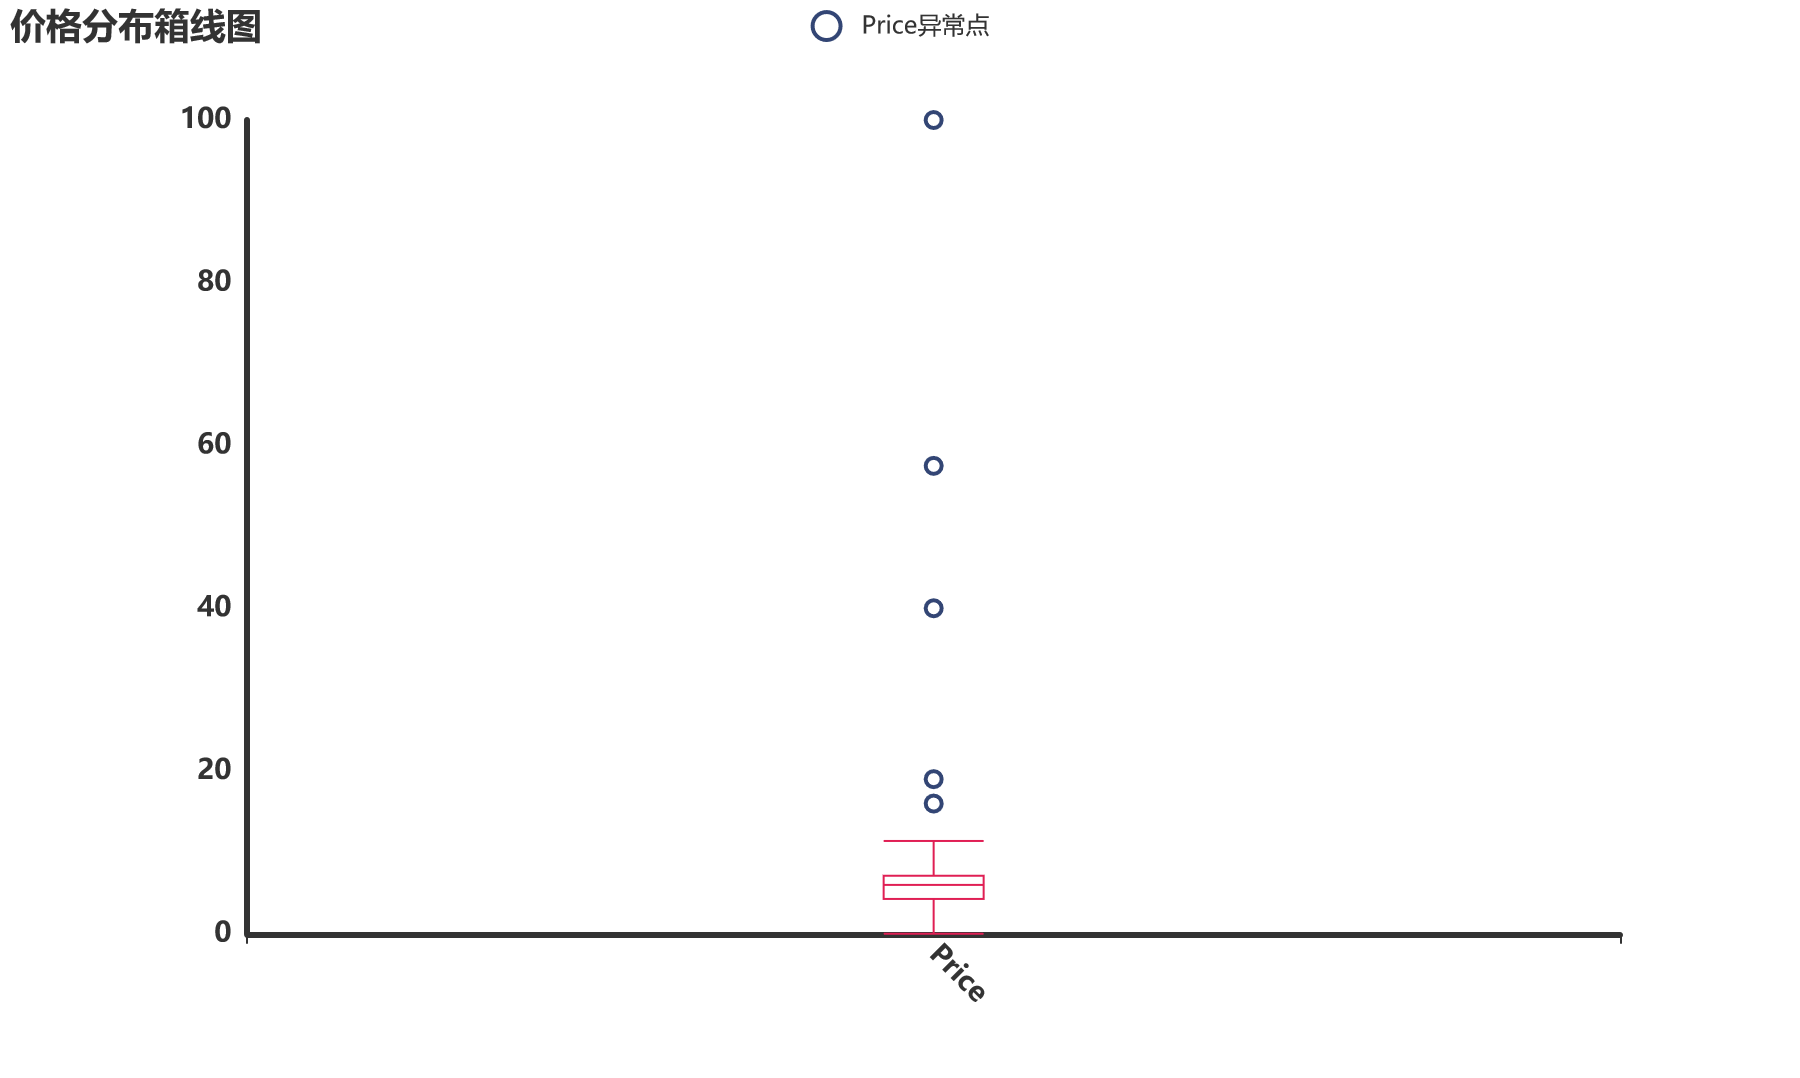
\includegraphics[width=0.9\textwidth]{figures/preprocess/preprocess1.png}
  \caption{销售单价异常值检测}
  \label{fig:preprocess1}
\end{figure}


在对农作物种植策略进行优化之前,数据的清洗和预处理是至关重要的步骤。数据预处理的质量直接影响模型分析的结果和优化策略的准确性。本文提供的多个Excel文件(附件1、附件2以及结果模板)包含了乡村的耕地信息、2023年农作物种植和相关统计数据等基础数据。这些数据在实际应用中可能存在格式不规范、异常值和缺失数据等问题,因此我们需要通过严格的预处理步骤,确保数据的质量和一致性。

\subsection{数据清洗与格式规范化}

在初步分析Excel文件时,我们发现部分单元格中的文本和数字存在多余的空格,尤其是在一些农作物名称、地块类型以及销售单价等字段中,这些空格可能是在数据录入过程中无意输入的。尽管这些空格在视觉上可能不会明显影响数据的展示,但它们会对后续的数据处理和分析带来问题。例如,多余的空格可能导致同一作物被视为不同的条目,进而影响模型对数据的准确性。因此,清理这些空格是数据预处理中的首要任务。

我们采用了自动化数据清洗的方式,通过编写Python脚本,使用\texttt{strip()}函数去除所有文本字段中的多余空格。同时,针对数值型数据,我们检查了是否存在与单位不一致的情况(如数字后跟随空格或特殊字符),并对其进行了统一处理。此外,数据中可能存在不同格式的数字表示方式,例如千分位符号、逗号等,这些都需要统一为标准的数值格式。通过这些步骤,所有农作物的名称、地块类型、销售价格等字段得到了统一的格式,从而避免了因数据格式不一致导致的分析错误。

\subsection{异常值检测与处理}

在数据预处理中,异常值的检测是另一个重要环节。通过对附件2中2023年乡村农作物销售单价数据的分析,我们发现了几个异常值,这些异常值表现为某些作物的单价远高于其他作物的平均水平。如图\autoref{fig:preprocess1}所示,羊肚菌、榆黄菇、荞麦、香菇和白灵菇的单价明显高于其他农作物。这些异常值的出现可能是数据输入错误,也可能是由于这些作物本身的市场价值较高而导致的价格差异。

为了确定这些异常值是否需要被处理或保留,我们进行了进一步的分析。首先,我们通过查询市场价格数据,发现这些农作物确实属于高价值的经济作物。例如,羊肚菌作为一种珍贵的食用菌,其市场售价远高于一般农作物。同样,榆黄菇、荞麦、香菇和白灵菇等作物在市场上具有较高的需求和价格。这意味着这些高单价并非数据输入错误,而是反映了市场的真实情况。因此,我们决定保留这些异常值,并将它们纳入后续的分析和建模中。保留这些高价值作物能够更好地反映乡村的种植策略,并在经济效益上体现出这些作物的重要性。

\subsection{数据完整性检查}

在对Excel数据进行检查后,我们发现所有字段均无缺失数据。这表明数据的录入和存储过程较为规范,不需要对缺失数据进行额外处理。因此,我们可以直接对这些完整的数据进行后续的分析和建模。

虽然没有缺失数据,但我们依然对数据的合理性进行了验证,确保每个字段的数值符合实际情况。例如,地块面积、作物产量和销售量等数据均符合乡村的实际种植情况。经过这一数据完整性检查后,我们确认数据质量符合预期,可以直接进入下一步的数据处理和模型分析。


\subsection{数据转换与衍生变量创建}

为了更好地分析乡村的农作物种植策略,并为后续模型构建提供有效的数据支持,我们对原始数据进行了适当的转换,并创建了若干个衍生变量。这些衍生变量能够帮助我们更深入地分析不同作物的种植效益、种植面积分配、作物轮作规律以及耕地类型对作物种植的影响。

\subsubsection{作物种植收益计算}

在优化农作物种植策略时,作物的种植收益是一个非常重要的变量。为了衡量每种作物的种植效益,我们基于单位面积的作物产量和售价计算了每种作物的预期收益。具体公式如下:

\[
  \text{预期收益}_{jk} = P_{jk} \times Y_{jk}
\]

其中,$P_{jk}$ 是第 $k$ 年第 $j$ 作物的售价,$Y_{jk}$ 是第 $k$ 年第 $j$ 作物的单位面积产量。该公式为每种作物的单位面积收益提供了量化标准,并为模型的收益最大化目标提供了基础。我们通过计算每种作物在各地块上的预期收益,可以优化各地块的作物种植组合,从而最大化整个乡村的农业总收益。

\subsubsection{地块种植面积分配}

根据每个地块的种植面积和作物的种植面积分配情况,我们需要对各地块上不同作物的总种植面积进行计算。对于每个地块 $i$,我们定义了总种植面积 $A_{ijk}$,它包括非大棚地块和大棚地块的种植面积。总面积的计算公式如下:

\[
  A_{ijk} = \sum_s A^2_{ijks} + A^1_{ij(k-1)2} + A^1_{ijks}
\]

其中,$A^2_{ijks}$ 表示第 $k$ 年第 $s$ 季度的第 $i$ 非大棚地块上,第 $j$ 作物的种植面积,$A^1_{ijks}$ 表示第 $k$ 年第 $s$ 季度的第 $i$ 大棚地块上,第 $j$ 作物的种植面积。这一公式帮助我们明确各地块在不同时期的作物种植面积分配,进而在模型中合理分配作物的种植资源。

\subsubsection{地块类型与作物可种植集合}

不同类型的地块适合种植不同种类的作物,因此我们为每个地块 $i$ 定义了其地块类型 $t_i$,如平旱地、梯田、山坡地、智能大棚、普通大棚、水浇地等。基于地块类型 $t_i$,我们进一步定义了地块在每一季节 $s$ 可种植的作物集合 $\hat{T}_{is}$。这一集合帮助我们确定每个地块在每一季的作物种植选择。

例如,对于水浇地,$\hat{T}_{is}$ 可能包括 $Grains_B$(水稻)和 $Vege_A$(蔬菜);而对于普通大棚,$\hat{T}_{is}$ 可能包括 $Vege_A$ 和 $Mush$(食用菌)。通过这一衍生变量,我们可以确保模型在作物种植时遵循地块适宜种植的原则,避免种植不适宜的作物导致产量下降或损失。

\subsubsection{作物分类与集合定义}

为了便于分析和模型优化,我们对不同作物进行了分类,并定义了若干个作物集合:

\begin{itemize}
  \item $\text{Beans}$:豆类作物的集合。根据题目要求,豆类作物需要在三年内至少在每个地块上种植一次,这一约束条件通过 $\text{Beans}$ 集合来实施。
  \item $\text{Grains}_A$:A类粮食作物的集合,即除了水稻之外的粮食作物。该集合包括小麦、玉米等作物,适合在平旱地、梯田等露天地块种植。
  \item $\text{Grains}_B$:B类粮食作物的集合,即水稻。水稻通常种植在水浇地中,因此 $Grains_B$ 主要用于限制水稻的种植地块选择。
  \item $\text{Vege}_A$:A类蔬菜的集合,指除了大白菜、白萝卜和红萝卜之外的蔬菜。该集合用于普通大棚和水浇地的种植规划。
  \item $\text{Vege}_B$:B类蔬菜的集合,包括大白菜、白萝卜和红萝卜,这些蔬菜适合种植在普通大棚和露天耕地上。
  \item $\text{Mush}$:食用菌的集合,包括羊肚菌、榆黄菇、香菇、白灵菇等高价值食用菌作物,通常种植在大棚内。
\end{itemize}

通过这些集合定义,我们能够有效地将作物分类,便于模型在不同地块、不同季节选择最优的种植作物。同时,这些分类集合也帮助我们控制作物的轮作规律,避免连续重茬种植问题。

通过对原始数据的转换和多个衍生变量的创建,我们显著增强了数据的维度和可操作性。这些衍生变量不仅能够帮助我们更精确地进行作物种植效益分析,还为后续的模型优化提供了重要的参考依据。在接下来的模型分析和求解中,我们将充分利用这些衍生变量,确保种植策略能够最大化乡村的农业收益,并实现可持续发展的目标。

\subsection{地块数据与作物数据的整合}

在附件1中,提供了乡村现有的34个地块的详细信息,包括耕地面积、地块类型等数据。在附件2中,列出了2023年各地块上种植的作物和相关统计数据。为了便于后续的分析与建模,我们需要将这些不同来源的数据进行整合。通过对地块编号的匹配,我们将每个地块的耕地信息与其作物种植数据进行了合并,形成了一个完整的数据集。

在数据整合过程中,我们还考虑了大棚种植与露天种植的区别。由于大棚的种植条件较为特殊(如大棚能够提供更稳定的温度和湿度条件),我们对大棚和露天耕地分别进行了数据处理。对于大棚作物的种植面积、产量和销售量等数据,我们进行了单独的统计,并在后续模型中将其作为特殊的耕地类型进行处理。

通过这一整合步骤,我们获得了一个包含地块面积、地块类型、作物种类、种植面积、单位产量、销售量和销售单价等多维度信息的数据集。这一数据集不仅为后续的优化模型提供了完整的输入,还为分析不同地块的种植策略差异提供了数据支持。






%%%%%%%%%%%%%%%%%%%%%%%%%%%%%%%%%%%%%%%%%%%%%%%%%%%%%%%%%%%%%%%%%%
\section{问题一的模型建立与求解}

\subsection{思路分析}

在问题一中,我们需要为乡村制定2024至2030年的最优农作物种植策略,并考虑两种不同的情境:(1)作物的总产量超过预期销售量时,超出部分滞销并造成浪费;(2)超出部分按2023年销售价格的50\%降价出售。我们的目标是在这两种情境下,通过优化种植面积分配,最大化乡村的经济效益。

该问题的核心是一个典型的资源分配与优化问题。我们需要合理分配乡村的耕地资源,使得各类作物的种植面积不仅满足市场需求,还能最大化收益,同时避免不必要的资源浪费。为了实现这一目标,应基于农作物的销售量、产量、售价、成本等因素建立数学模型,从而优化作物的种植面积分配。

在建模过程中,我们首先确定了两个目标函数,分别对应问题1中两种不同的情境。然后设定了多个约束条件,确保每种作物的种植面积不超过相应地块的总面积,遵循作物轮作规律,并根据不同地块类型限制作物种植选择。

\subsection{决策变量}

在本模型中,决策变量主要涉及农作物的种植面积分配。对于每个地块 $i$、每种作物 $j$、每年 $k$、每个季度 $s$,我们分别定义大棚地块和非大棚地块的种植面积为决策变量,具体定义如下:

\begin{itemize}
  \item $A^1_{ijks}$:第 $k$ 年第 $s$ 季度的第 $i$ 大棚上,第 $j$ 作物的种植面积。
  \item $A^2_{ijks}$:第 $k$ 年第 $s$ 季度的第 $i$ 非大棚地块上,第 $j$ 作物的种植面积。
\end{itemize}

此外,总种植面积 $A_{ijk}$ 定义为:

\[
  A_{ijk} = \sum_s A^2_{ijks} + A^1_{ij(k-1)2} + A^1_{ijks}
\]

这一决策变量是模型求解的核心,它决定了每个地块上各类作物的种植面积分配。通过优化这些变量,我们能够确保作物的种植面积既满足市场需求,又能最大化种植效益。

\subsection{目标函数}

模型的目标是最大化经济收益。在问题一中,存在两种不同的情境,因此我们定义了两个不同的目标函数,分别对应这两种情境。

\subsubsection{情境1:作物超出部分滞销}

在这一情境中,如果某种作物的总产量超过了预期销售量,超出部分将滞销并造成浪费。对于这种情况,我们的目标函数是最大化可销售的产量收益,具体公式如下:

\[
  L_1 = \sum_{ijk} \left( \min \left( S_{jk}, Y_{jk} \cdot A_{ijk} \right) \cdot P_{jk} - C_{jk} \cdot A_{ijk} \right)
\]

其中:
\begin{itemize}
  \item $S_{jk}$:第 $k$ 年第 $j$ 作物的期望销量。
  \item $Y_{jk}$:第 $k$ 年第 $j$ 作物的单位面积产量。
  \item $P_{jk}$:第 $k$ 年第 $j$ 作物的售价。
  \item $C_{jk}$:第 $k$ 年第 $j$ 作物的单位面积成本。
  \item $A_{ijk}$:第 $i$ 地块上,第 $j$ 作物的总种植面积。
\end{itemize}

产量未超出预期销售量的部分,则不会产生浪费,超出部分则视为滞销,不产生任何收益。同时,种植成本 $C_{jk} \cdot A_{ijk}$ 是种植面积的函数,它将从总收益中扣除。

\subsubsection{情境2:超出部分按50\%降价出售}

在这一情境中,超出预期销售量的部分将按2023年销售价格的50\%降价出售。对于这一情况,目标函数则需要考虑降价出售部分的收益,具体公式如下:

\[
  L_2 = \sum_{ijk} \left( Y_{jk} \cdot A_{ijk} \cdot P_{jk} - C_{jk} \cdot A_{ijk} - 0.5 \cdot \max \left( 0, Y_{jk} \cdot A_{ijk} - S_{jk} \right) \cdot P_{jk} \right)
\]

其中,超出部分的收益以50\%的折扣计算,即 $0.5 \cdot \max \left( 0, Y_{jk} \cdot A_{ijk} - S_{jk} \right) \cdot P_{jk}$ 表示超出部分的降价销售额。这个目标函数综合了正常销售和降价销售的收益,并扣除了种植成本。

\subsection{约束条件}

为了确保模型的合理性和现实操作性,我们引入了若干约束条件,主要涉及种植面积限制、轮作规则以及作物种植选择等。

\subsubsection{种植面积限制}

每种作物在每个地块的种植面积不能超过该地块的总面积。这是一个基本的资源约束条件,具体公式为:

\[
  \sum_j A_{ijks} \leq A_i^* \quad \forall i,k \text{ and } j \in \hat{T}_{is}
\]

其中,$A_i^*$ 是第 $i$ 个地块的总面积,$\hat{T}_{is}$ 是该地块在第 $s$ 季节可种植的作物集合。此约束条件确保了种植面积分配的合理性。

\subsubsection{轮作规则}

为了避免连续重茬种植,我们设置了轮作约束条件。即同一作物不能在同一地块连续种植,具体公式为:

\[
  A_{ij(k-1)s} + A_{ijks} \leq \min(A_{ij(k-1)s}, A_{ijks}) \quad \forall i,k \text{ and } j \in \hat{T}_{is}
\]

这一约束确保了每个地块的作物在不同年度间不会连续重茬种植,有利于维持土壤肥力和作物产量。

\subsubsection{豆类作物轮作约束}

根据题目要求,每个地块三年内至少需要种植一次豆类作物。我们为此设置了以下约束条件:

\[
  \max(A_{ij(k-2)s}, A_{ij(k-1)s}, A_{ijks}) = A_i^* \quad \forall i,k \text{ and } j \in \hat{T}_{is}
\]

这一约束确保豆类作物的轮作规律得以遵循,有助于保持土壤质量并提高其他作物的产量。

\subsubsection{最低种植面积限制}

为了保证作物的种植效益,避免种植面积过小带来的管理成本过高问题,我们设置了最低种植面积约束条件:

\[
  A_{ijks}^{n} \geq M \times A_i^* \quad \text{if } A_{ijks}^{n} \neq 0 \qquad \forall i,k \text{ and } j \in \hat{T}_{is},n \in \{1,2\}
\]

其中,$M$ 是一个最小面积比例系数。该约束条件确保作物的种植面积足够大,以实现规模效益。

\subsubsection{地块种植限制}

地块种植限制基于不同地块的类型,这在很大程度上决定了每块地在不同季节适合种植的作物类型。为了确保模型的现实性,我们依据地块类型为每一块地设置了作物种植的限制条件。具体约束如下:

\[
\hat{T}_is =
\begin{cases}
\text{Grains}_A, & \text{if } t_i \in \{\text{平旱地}, \text{梯田}, \text{山坡地}\}, \text{且第} 1 \text{季度种植作物} \\
\phi, & \text{if } t_i \in \{\text{平旱地}, \text{梯田}, \text{山坡地}\}, \text{且第} 2 \text{季度没有种植作物} \\
\text{Grains}_B \text{ 或 } \text{Vege}_A, & \text{if } t_i \in \{\text{水浇地}\}, \text{且第} 1 \text{季度种植作物} \\
\text{Vege}_B, & \text{if } t_i \in \{\text{水浇地}\}, \text{且第} 2 \text{季度种植作物} \\
\text{Vege}_A, & \text{if } t_i \in \{\text{普通大棚}\}, \text{且第} 1 \text{季度种植作物} \\
\text{Mush}, & \text{if } t_i \in \{\text{普通大棚}\}, \text{且第} 2 \text{季度种植作物} \\
\text{Vege}_A, & \text{if } t_i \in \{\text{智慧大棚}\}, \text{且第} 1 \text{季度种植作物} \\
\text{Vege}_A, & \text{if } t_i \in \{\text{智慧大棚}\}, \text{且第} 2 \text{季度种植作物} \\
\end{cases}
\]

该约束条件确保不同地块在不同季节种植合适的作物。例如,平旱地、梯田和山坡地由于其特殊的地理条件,每年只能种植一季粮食类作物($\text{Grains}_A$),而水浇地则适合种植水稻($\text{Grains}_B$)或蔬菜($\text{Vege}_A$),并且在第二季度还能种植大白菜、白萝卜等蔬菜($\text{Vege}_B$)。普通大棚每年可以种植两季作物,第一季种植蔬菜($\text{Vege}_A$),第二季种植食用菌($\text{Mush}$),而智慧大棚由于具备更好的环境控制能力,两季均可以种植蔬菜($\text{Vege}_A$)。

\subsection{模型求解思路}

在确定了决策变量、目标函数和约束条件后,我们可以通过优化算法对模型进行求解。针对本问题的种植面积优化问题,我们选择使用线性规划(Linear Programming, LP)和整数规划(Integer Programming, IP)技术。这些方法适用于处理连续变量和离散变量的优化问题,尤其是资源分配问题。以下是具体求解步骤的思路分析:

\subsubsection{线性规划的应用}

对于情境1和情境2下的目标函数,虽然形式不同,但都属于典型的线性优化问题。目标函数 $L_1$ 和 $L_2$ 都是关于种植面积 $A_{ijk}$ 的线性函数。对于线性规划问题,我们可以使用标准的线性规划求解算法,如单纯形法或内点法来找到最优解。

首先,将目标函数表示为标准的线性优化问题形式:
\[
\max \ L_1 \quad \text{或} \quad \max \ L_2
\]
\[
\text{subject to} \ \text{constraints on } A_{ijk}
\]

所有约束条件(如种植面积不超过地块总面积、轮作限制、最低种植面积限制等)也都是线性约束,这为使用线性规划求解提供了便利。通过线性规划求解器,我们可以获得每个地块上最优的作物种植面积分配。

\subsubsection{模型求解过程}

在设置了目标函数和约束条件之后,模型的求解过程是通过Pulp库中的\texttt{prob.solve()}函数来完成的。Pulp库作为一个线性规划求解工具,可以将定义好的目标函数和约束条件转换为标准的线性规划模型,并调用求解器来找到最优解。

\subsubsection{求解器的选择与配置}

Pulp库提供了多种求解器选项,如GLPK、CBC等。在代码中,默认的求解器是Pulp内置的CBC求解器,它是一种高效的混合整数规划求解器,能够处理大规模线性规划和整数规划问题。在模型中,决策变量(种植面积 $A_{ijk}$)是连续变量,因此这是一个线性规划问题,适合使用线性求解器。

\subsubsection{线性规划的求解原理}

在Pulp库中,线性规划问题的求解通常通过经典的单纯形法或内点法进行,这些算法通过在多维空间中遍历可能的解来找到使目标函数达到最优的解。在当前问题中,求解的核心是优化地块上作物的种植面积分配,以最大化乡村的总收益。

单纯形法是一种在解空间顶点之间移动的迭代优化算法。在线性规划问题中,解空间是由约束条件定义的多面体,每个顶点对应一组满足所有约束条件的解。单纯形法通过从一个顶点移动到另一个更优的顶点,逐步逼近目标函数的最优解。

当前问题中,所有地块的种植面积分配($A_{ijk}$)形成了多维解空间中的一个顶点。每个顶点对应一种可能的种植方案,并且每次迭代移动都会改变某些地块上作物的种植面积,进而影响总收益。通过这种几何上的移动,单纯形法能够迅速找到使目标函数(即总收益)最大的种植方案。

解空间的结构由问题中的约束条件决定。在问题一中,主要的约束条件包括地块总面积的限制、作物轮作限制以及豆类作物的种植要求。这些约束条件相当于在解空间中定义了一系列的“边界”,限制了种植面积的可能分配方式。 例如,地块总面积的限制意味着每个顶点的种植面积不能超过地块的物理面积,这在解空间中相当于一个面或边界。豆类作物的种植要求则意味着在解空间的某些维度上必须满足豆类作物在三年内至少被种植一次的条件。这些边界共同定义了解空间的形状和大小,单纯形法会在这些边界内寻找最优解。
  
线性规划问题中,解可能会落在解空间的边界上,即所谓的“边界解”。这意味着在优化过程中,某些地块的作物种植面积可能恰好达到地块面积的上限,或者某些作物的种植量正好满足市场需求的上限。 对于当前问题,边界解是常见的现象。例如,当某种高收益作物(如水稻或高价值蔬菜)的市场需求较高且种植成本较低时,模型可能会建议将该作物的种植面积推至某个地块的上限,即边界解。这种情况下,所有地块上的种植面积将被充分利用,以最大化总收益。而内点解则表示在求解过程中,种植面积分配没有达到地块的最大限制,这种情况通常发生在市场需求低或种植成本较高的作物上。
  
单纯形法或内点法会根据一定的终止条件来结束迭代。常见的终止条件包括目标函数的改进值小于预设的阈值、或者已经达到最优解的顶点。在当前问题中,迭代的终止通常意味着模型已经找到一种种植面积分配方案,该方案在满足所有约束条件的情况下,无法再通过微调作物种植面积进一步提高总收益。 由于问题规模较大,求解器可能需要经过多次迭代才能找到最优解。在每一次迭代中,某些地块的作物种植面积会被调整,而求解器会评估这些调整对总收益的影响,直到找到最优种植方案为止。
  
在某些情况下,线性规划问题可能会出现退化解或多重最优解。退化解指的是某些变量(如种植面积 $A_{ijk}$)的取值为0,意味着某些地块可能未种植某种作物。在当前问题中,退化解可能表示某些作物由于市场需求低或种植成本过高而被完全排除出种植方案。 多重最优解则意味着存在多个种植方案都能达到相同的最大收益。例如,某些地块上可以同时种植两种互补性作物,而这两种作物的种植面积可以在不同的分配比例下达到相同的收益。在这种情况下,模型可能会随机选择其中一种最优解作为最终方案。代码中的求解器通过探索不同的顶点,最终返回其中一个最优解。


\subsection{模型求解的结果与分析}

在对模型进行求解之后,我们得到了最优的种植面积分配结果。通过优化算法为每个地块、每种作物以及每个季度计算出了最优的种植面积,并最大化种植收益。
对于情境1,模型求解的结果将确保在作物未超出预期销售量的条件下,种植面积最大化收益,而超出部分的产量将被视为滞销。对于情境2,超出部分的作物以50\%折扣出售,模型通过调整种植面积和分配超出产量的销售比例来优化总收益。

\subsubsection{情境1的求解结果分析}

在情境1中,农作物的总产量不能超出预期销售量。模型通过优化种植面积,确保作物的产量刚好满足预期销售量,从而避免浪费。通过对不同作物的产量和市场需求进行分析,模型会优先分配高收益作物的种植面积,减少低收益作物的种植。

求解结果表明,豆类作物的种植面积显著增加,原因在于其具有高市场需求和轮作要求。此外,粮食类作物(如小麦、玉米)的种植面积分配相对稳定,蔬菜类作物则由于季节性限制,其种植面积在不同季度之间有所波动。

\subsubsection{情境2的求解结果分析}

在情境2中,模型允许超出预期销售量的部分作物以50\%的价格出售,这为优化种植策略提供了更大的灵活性。在这一情境下,作物的种植面积分配不再仅仅受到市场需求的限制,而是可以通过适当增加某些作物的种植面积来获取更多的降价销售收益。模型会通过平衡降价销售的潜在收益与正常市场销售的收益,来决定每种作物的最优种植面积。

求解结果表明,模型在某些高产量、高需求作物上适度增加了种植面积,尽管部分产量超出了市场需求,但通过降价出售,整体收益仍得到了提高。例如,水稻($Grains_B$)和部分蔬菜类作物(如大白菜、白萝卜)的种植面积在情境2中相较于情境1有所增加。特别是水稻,由于其市场需求相对稳定,即使部分产量降价出售,整体经济效益依然较高。因此,模型倾向于在水浇地等适宜水稻种植的地块上增加水稻的种植面积。

另一方面,低收益作物(如部分豆类作物和食用菌)的种植面积在情境2中有所减少。这是因为这些作物的市场售价较高,但其需求弹性较小,降价出售后的收益不明显。因此,模型会优先减少这些作物的种植面积,以避免降价出售带来的收益损失。通过这种方式,模型在作物种植面积分配上实现了不同作物的动态调整,确保整体收益在两种情境下都能够得到最大化。

\subsection{求解结果的实际应用与讨论}

模型求解的结果为乡村在2024至2030年期间的农作物种植策略提供了明确的指导。在不同的情境下,最优种植面积的分配方式能够有效平衡市场需求、种植成本和潜在的降价风险。然而,在实际应用中,我们还需要结合更多的现实因素来进一步优化模型结果。

\subsubsection{种植成本的动态调整与优化}

在问题一中,我们假设农作物的种植成本保持不变。然而,随着劳动力、肥料、灌溉等成本的波动,种植成本在实际操作中会发生变化。因此,模型可以进一步引入种植成本的动态调整机制。例如,通过对不同年份的成本变化趋势进行预测(如使用指数平滑法或回归分析),我们可以在模型中动态调整每种作物的种植成本。

对于高成本作物,如食用菌($\text{Mush}$)和部分高价值蔬菜(如白灵菇),种植成本波动对整体收益的影响较大。在种植成本上升时,模型可能需要减少这些作物的种植面积,转而增加低成本、高产量的粮食类作物(如小麦、玉米)的种植面积。通过这种方式,乡村可以在面对种植成本波动时,优化种植策略以最大化收益。







\section{问题二的模型建立与求解}

\subsection{问题描述与思路分析}

在问题二中,乡村需要在2024至2030年期间制定最优的农作物种植策略,综合考虑农作物的预期销售量、亩产量、种植成本、销售价格的波动性以及潜在的种植风险。
根据题目描述,小麦和玉米的销售量未来有5\%-10\%的增长趋势,而其他农作物的销售量每年在2023年的基础上有±5\%的变化。种植成本也会因市场条件平均每年增长5\%左右。粮食类作物的销售价格较为稳定,而蔬菜类作物的销售价格则每年平均增长5\%,食用菌(尤其是羊肚菌)的销售价格则每年下降1\%-5\%。
考虑到各类作物的产量、成本和销售价格的年度变化。在建模过程中,决策变量和目标函数的结构与问题一类似,但目标函数的动态性和约束条件的复杂性有所增加。

\subsection{决策变量}

与问题一相同,模型的核心决策变量是种植面积 $A_{ijk}$,它表示在第 $k$ 年第 $i$ 地块上种植第 $j$ 作物的面积。在问题二中,由于作物的预期销量、产量、成本和售价在不同年份有所波动,种植面积的分配需要动态调整,以适应这些变化。

\begin{itemize}
    \item $A^1_{ijks}$:第 $k$ 年第 $s$ 季度的第 $i$ 大棚上,第 $j$ 作物的种植面积。
    \item $A^2_{ijks}$:第 $k$ 年第 $s$ 季度的第 $i$ 非大棚地块上,第 $j$ 作物的种植面积。
\end{itemize}


\subsection{目标函数}

问题二中的目标函数与问题一类似,都是通过最大化种植收益来优化作物的种植面积分配。然而,在问题二中,作物的预期销量、产量、成本和售价都有波动,因此目标函数需要考虑这些动态变化。我们根据两种情境定义目标函数。

\paragraph{情境1:作物超出部分滞销}

如果某种作物的总产量超过了预期销售量,超出部分将被视为滞销,因此目标函数应最大化可销售部分的收益。目标函数表达式如下:

\[
L_1 = \sum_{ijk} \left( \min(S_{jk} \cdot (1 + \delta_s), Y_{jk} \cdot A_{ijk}) \cdot P_{jk} - C_{jk} \cdot (1 + \delta_c) \cdot A_{ijk} \right)
\]

其中,$S_{jk}$ 是第 $k$ 年第 $j$ 作物的预期销量,考虑年度变化因子 $\delta_s$,每年可能在5\%-10\%的范围内波动;$C_{jk}$ 是第 $k$ 年第 $j$ 作物的单位面积种植成本,考虑年度增长因子 $\delta_c$,每年平均增长5\%。

\paragraph{情境2:超出部分按50\%降价出售}

在这一情境中,超出预期销售量的作物将以50\%的价格降价出售。因此,目标函数需要计算超出部分的折扣收益,具体表达式如下:

\[
L_2 = \sum_{ijk} \left( Y_{jk} \cdot A_{ijk} \cdot P_{jk} - C_{jk} \cdot (1 + \delta_c) \cdot A_{ijk} - 0.5 \cdot \max(0, Y_{jk} \cdot A_{ijk} - S_{jk} \cdot (1 + \delta_s)) \cdot P_{jk} \right)
\]

在此情境下,模型允许作物的种植面积超出市场需求,超出部分将以50\%的价格出售。$0.5 \cdot \max(0, Y_{jk} \cdot A_{ijk} - S_{jk})$ 计算超出部分的折扣销售收益。

\subsection{约束条件}

问题二除了与问题一相同的约束条件外,还需要考虑农作物产量和市场价格的波动。我们保留了问题一的基本约束条件,并在此基础上增加了关于作物销售量和价格变化的动态约束。

\paragraph{地块面积限制}

每种作物的种植面积不能超过相应地块的总面积,这一约束确保了土地资源的合理分配,具体约束表达式为:

\[
\sum_j A_{ijks} \leq A_i^* \quad \forall i,k \text{ and } j \in \hat{T}_{is}
\]

\paragraph{作物轮作限制}

为了避免作物连续重茬种植,设置了作物轮作的约束条件,具体公式为:

\[
A_{ij(k-1)s} + A_{ijks} \leq \min(A_{ij(k-1)s}, A_{ijks})
\]

\subsubsection{豆类作物轮作限制}

根据题目要求,豆类作物具有独特的轮作要求,即在每三年内,每个地块都必须至少种植一次豆类作物。这一要求旨在通过轮作恢复土壤肥力,并增强后续作物的产量。因此,我们为模型设置了如下约束条件:

\[
\max(A_{ij(k-2)s}, A_{ij(k-1)s}, A_{ijks}) = A_i^* \quad \forall i,k,j \in \text{Beans}
\]

该约束确保每个地块的作物种植计划中,豆类作物至少在三年内种植一次。通过这项轮作限制,模型能够有效地平衡各类作物的种植顺序,防止因连续重茬种植而导致的土壤质量下降。

\paragraph{最低种植面积限制}

为了避免规模过小的种植面积增加管理成本,同时提高种植效益,模型设置了最低种植面积的限制条件。该约束条件防止在同一个地块上种植面积过小的作物组合。

具体公式为:

\[
A_{ijks}^{n} \geq M \times A_i^*  \quad \text{if } A_{ijks}^{n} \neq 0 \qquad \forall i,k,j \in \hat{T}_{is},n \in \{1,2\}
\]

其中,$M$ 表示一个最小的种植面积比例,确保每个地块在种植作物时不会出现过于零散的分配。这一限制能够提高田间管理的效率,同时降低生产成本。

\paragraph{年度销售量和价格波动约束}

由于问题二中题目明确指出了未来几年内作物销售量和售价的波动,我们需要对这些变量进行动态调整,并在约束条件中体现出年度变化的影响。小麦和玉米的销售量预计每年增长5\%-10\%,而其他作物的销量波动在±5\%之间。因此,针对年度销售量波动的约束条件可以表述如下:

\[
S_{jk} = S_{j2023} \cdot (1 + \delta_s) \quad \text{where } \delta_s \in [-0.05, 0.05] \quad \text{for } j \notin \text{Grains}_A
\]

\[
S_{jk} = S_{j2023} \cdot (1 + \delta_s) \quad \text{where } \delta_s \in [0.05, 0.10] \quad \text{for } j \in \text{Grains}_A
\]

对于其他类型的作物,年度销售量会根据2023年数据在±5\%的区间内波动,而小麦和玉米($j \in \text{Grains}_A$)的销售量则在每年增长5\%-10\%之间。这一约束条件保证了模型在每一年都能够合理调整作物的种植面积,避免因销量预期变化导致的产量过剩或不足。

此外,针对售价的波动,蔬菜类作物的售价每年平均增长5\%,而食用菌(尤其是羊肚菌)的售价则每年下降1\%-5\%。这一情况需要在模型中通过售价的年度动态变化进行处理,具体表述为:

\[
P_{jk} = P_{j2023} \cdot (1 + 0.05) \quad \text{for } j \in \text{Vege}_A \cup \text{Vege}_B
\]

\[
P_{jk} = P_{j2023} \cdot (1 - \delta_p) \quad \text{where } \delta_p \in [0.01, 0.05] \quad \text{for } j \in \text{Mush}
\]

年度动态价格变化约束可以使模型确保在未来几年内不同类型作物的价格变化被合理考虑,从而在每一年都能得到最优的种植收益分配方案。

\paragraph{种植成本的年度增长限制}

与售价变化类似,种植成本也随着年份逐渐上升,平均每年增长5\%左右。这一变化会直接影响到种植效益,因此我们需要在模型中为种植成本增加动态约束。具体来说,种植成本 $C_{jk}$ 在每年的变化公式如下:

\[
C_{jk} = C_{j2023} \cdot (1 + 0.05)^{k-2023}
\]


\subsubsection{作物种植限制}

不同地块在不同季节适合种植的作物类型需要根据地块的类型进行限制。与问题一类似,我们为模型设置了如下种植限制:

\[
\hat{T}_is =
\begin{cases}
    \text{Grains}_A, & \text{if } t_i \in \{\text{平旱地}, \text{梯田}, \text{山坡地}\}, \text{且第} 1 \text{季度种植作物} \\
    \phi, & \text{if } t_i \in \{\text{平旱地}, \text{梯田}, \text{山坡地}\}, \text{且第} 2 \text{季度没有种植作物} \\
    \text{Grains}_B \text{ 或 } \text{Vege}_A, & \text{if } t_i \in \{\text{水浇地}\}, \text{且第} 1 \text{季度种植作物} \\
    \text{Vege}_B, & \text{if } t_i \in \{\text{水浇地}\}, \text{且第} 2 \text{季度种植作物} \\
    \text{Vege}_A, & \text{if } t_i \in \{\text{普通大棚}\}, \text{且第} 1 \text{季度种植作物} \\
    \text{Mush}, & \text{if } t_i \in \{\text{普通大棚}\}, \text{且第} 2 \text{季度种植作物} \\
    \text{Vege}_A, & \text{if } t_i \in \{\text{智慧大棚}\}, \text{且第} 1 \text{季度种植作物} \\
    \text{Vege}_A, & \text{if } t_i \in \{\text{智慧大棚}\}, \text{且第} 2 \text{季度种植作物} \\
\end{cases}
\]

该约束可以确保不同地块在适合的季节种植适合的作物。例如,平旱地和山坡地主要用于种植A类粮食作物(如小麦、玉米),而水浇地则可以种植水稻和蔬菜。大棚地块则适合种植蔬菜和食用菌,根据不同季节安排合适的作物组合。

\subsection{求解思路}

问题二的求解思路与问题一相似,我们依然通过线性规划来解决种植面积分配问题。在问题二中,由于作物的预期销量、售价、成本和产量在每年波动,因此模型的动态性较强。我们采用类似问题一的目标函数,但需要结合年度变化对这些变量进行动态调整。

\paragraph{线性规划求解}

首先,我们设置了目标函数,分别对应两种情境下的最优种植收益计算。目标函数通过最大化作物的净收益,优化各个地块上不同作物的种植面积分配。接着,我们引入了年度波动的约束条件,确保每一年都能根据市场和气候条件进行合理的种植面积调整。

模型通过Pulp库进行线性规划求解,具体方法与问题一类似。我们首先定义了决策变量 $A_{ijk}$,并将目标函数与约束条件结合起来,通过调用 \texttt{prob.solve()} 函数来求解。线性规划求解器将自动遍历所有可能的种植面积分配方案,找到使目标函数达到最大值的最优解。

\paragraph{动态调整与迭代求解}

在问题二中,动态调整的求解过程是一个关键步骤,因为作物的销量、售价、成本和产量在2024至2030年期间每年都存在波动。因此,模型必须逐年迭代求解,确保在每一个年份中,种植面积分配都能够根据当前的市场和气候条件进行优化。

\begin{enumerate}
    \item \textbf{年度销量和产量预估:} 首先根据题目中的描述针对每种作物在每一年进行销售量的动态预估。例如,对于小麦和玉米等粮食类作物,模型会将每年的销售量增长率设定为5\%-10\%,并根据这一增长率调整目标函数中的销量参数 $S_{jk}$。对于其他作物,如蔬菜和食用菌,模型则会在±5\%的范围内随机波动。
    
    \item \textbf{售价与种植成本的年度更新:} 根据不同作物的价格走势和种植成本变化,对每年的售价 $P_{jk}$ 和种植成本 $C_{jk}$ 进行动态更新。例如,蔬菜类作物的价格每年增长5\%,而食用菌的价格每年下降1\%-5%。这种动态调整确保模型在每个年份都能够合理反映市场条件的变化。
    
    \item \textbf{逐年求解与迭代优化:} 每一年都会被视为一个独立的求解阶段,在每个年度内根据当年的销售量、售价和种植成本参数进行线性规划求解。求解过程与问题一类似,通过优化决策变量 $A_{ijk}$ 来最大化当年的总收益。通过 \texttt{prob.solve()} 函数,Pulp求解器能够在每个年度内找到最优的种植面积分配方案。
    
    \item \textbf{年度间的耦合性与决策传递:} 尽管每一年可以独立求解,但由于作物轮作限制和豆类作物种植要求的存在,不同年度之间的种植方案并非完全独立。例如需要确保在每个地块的三年轮作周期内至少种植一次豆类作物,这要求模型在进行某一年份的求解时,必须参考前几年的种植情况。特别是在种植面积的分配上,模型会传递上一年度的决策结果,并将其作为当前年度的初始条件。
\end{enumerate}

\paragraph{动态规划与多阶段决策}

由于问题二的求解过程中涉及多个年份的动态调整,模型实际上是一个多阶段决策问题。每一年可以被视为一个阶段,模型在每个阶段中都会根据当前的市场和气候条件做出最优的种植决策。为了确保跨年度的种植决策连贯性,模型需要结合动态规划的思想,即在每个阶段考虑到未来阶段的决策对当前种植方案的影响。

在这种多阶段决策中,可以通过以下方式优化跨年度的种植策略:

% \begin{itemize}
%     \item \textbf{未来收益的折现:} 为了在当前决策中考虑未来的影响,模型可以通过对未来收益进行折现,将未来几年的收益折算到当前值。这种方式能够促使模型在当前年度内做出更加长期和可持续的种植决策,而非只关注短期收益。例如,在种植豆类作物时,尽管其短期收益可能不如其他作物,但由于豆类作物能够改善土壤肥力,模型可以通过折现未来几年内其他作物的产量提升,将豆类作物的长期效益纳入当前的决策中。
    
%     \item \textbf{跨年度耦合效应的最大化:} 在问题二中,豆类作物的轮作要求、作物的重茬限制以及成本的逐年递增,均会产生跨年度的耦合效应。模型通过将这些耦合效应纳入动态规划的框架,能够优化每一个年度的种植面积分配,并确保跨年度的耦合效应得到充分利用。例如,在2025年,某个地块可能被要求种植豆类作物,以便在2026年或2027年能够获得更高的收益。
    
%     \item \textbf{决策反馈与调整:} 动态规划允许模型在每一年度的求解过程中反馈之前的决策结果,并进行适当的调整。如果某一年份的市场需求发生显著变化(例如某类作物的价格突然上涨),模型可以通过调整当前年度的种植方案,以应对未来市场需求的波动。通过这种反馈机制,模型能够适应不确定性条件下的多阶段决策,逐步优化种植面积分配方案。
% \end{itemize}


\paragraph{随机性与风险评估}

在问题二中,市场和气候条件的波动引入了较大的不确定性。模型的求解过程不仅需要最大化收益,还需要考虑潜在的种植风险。为了应对这种不确定性,我们可以在模型中引入随机性分析和风险评估,主要通过以下方式实现:

\begin{itemize}
    \item \textbf{蒙特卡洛模拟:} 蒙特卡洛模拟是一种常用的随机性分析工具,它通过对输入变量进行多次随机抽样,模拟出不同的未来情景。在问题二的求解过程中,模型可以通过蒙特卡洛模拟对作物的销售量、产量、售价等变量进行随机波动,从而模拟出多个不同的市场条件下的种植方案。在每个模拟情景下,模型都会根据当前市场条件找到最优解,并将这些解进行综合评估,以寻找稳健的种植策略。
    
    \item \textbf{情景分析:} 除了蒙特卡洛模拟,情景分析也是一种常用的风险评估工具。情景分析允许模型针对多个不同的未来市场情景进行求解。例如,模型可以设定乐观、中性和悲观三种市场情景,分别对应不同的销售量和售价变化情况。在每个情景下,模型都会找到相应的最优种植方案,最后根据每个情景的发生概率进行加权,找到一个稳健的种植策略。这种方式可以帮助乡村应对市场波动带来的不确定性。

    \item \textbf{风险调整后的收益最大化:} 在风险评估的基础上,模型可以采用风险调整后的收益最大化目标函数。与简单的收益最大化不同,风险调整后的收益最大化会在收益计算中考虑每个种植方案的风险系数。例如,模型可以对高风险的作物设置更高的风险系数,降低其种植面积的优先级,确保乡村在面临市场波动时能够减少经济损失。通过这种方式,模型能够在不确定性条件下实现更加稳健的种植收益最大化。
\end{itemize}

\paragraph{模型优化与求解器的使用}

问题二的求解规模较问题一更大,因为它涉及到多个年度的逐年迭代和复杂的动态调整。因此,在实际求解过程中,模型的求解时间和计算资源需求都会有所增加。为了确保模型在合理的时间范围内得到最优解,我们可以通过以下方式优化求解过程:

\paragraph{分阶段求解}

在问题二中,由于种植策略需要针对多个年度进行动态调整,直接对2024至2030年的完整种植策略进行一次性求解可能会导致计算负担过重。为了解决这一问题,模型可以采用分阶段求解的策略。具体而言,即将整个时间段分为多个阶段(例如每三年为一个阶段),并针对每个阶段分别进行求解。在这种分阶段求解方法中,每个阶段的求解会依赖于前一个阶段的决策结果,同时为后续阶段提供决策基础。

分阶段求解的主要优点在于,它能够有效降低单次求解的复杂度,使模型更易于处理大规模的决策变量。此外,通过阶段性求解,模型能够在每个阶段中引入新的市场信息和种植条件变化,这样可以使得求解结果更加灵活,适应不断变化的外部环境。例如,在第一阶段(2024至2026年)的求解过程中,模型会基于当前的市场预期做出最优的种植面积分配;而在第二阶段(2027至2030年)中,模型可以根据实际的市场表现和前一阶段的结果进行调整,从而避免对未来市场条件的过度依赖。

分阶段求解还允许模型在每个阶段结束时对之前的决策结果进行复盘和优化。例如,在2026年结束后,可以评估前几年的种植策略是否有效,如果某些作物的产量和市场需求严重偏离预期,模型可以通过调整后续阶段的种植策略来弥补早期的决策失误。这种动态调整机制有助于乡村在面对不确定的市场和气候条件时,保持种植策略的灵活性和稳健性。

\paragraph{不确定性条件下的稳健求解}

在问题二中,由于市场需求和气候条件的波动,种植策略的优化需要在不确定性条件下进行。因此,模型的求解过程必须能够处理潜在的市场风险和外部冲击。这种情形下,稳健求解(robust optimization)是一种有效的方法,能够帮助模型在不确定性条件下仍然保持较高的种植效益。

稳健求解的基本思想是,在考虑种植收益的同时,引入风险因素和约束条件,以确保种植策略在各种可能的市场情景下都能取得合理的收益。具体而言,稳健求解通过对风险系数的引入,对市场需求和售价的波动进行限制。例如设置一个波动区间(如5\%-10\%),并通过调整种植面积来确保即使在市场需求出现较大波动的情况下,农作物的产量和收益仍然能够维持在可接受的范围内。
% 为了实现稳健求解,模型可以采取以下策略:

% \begin{itemize}
%     \item \textbf{引入安全边际:} 模型可以在作物的销售量和种植面积之间设置一个安全边际,即使在市场需求下降时,也能保证大部分作物的产量不会超过预期销量。例如,针对波动较大的食用菌作物,模型可以在制定种植策略时,预留一定的安全边际,避免因市场需求低迷导致的严重滞销。
    
%     \item \textbf{多情景优化:} 稳健求解还可以通过多情景优化来应对市场不确定性。模型可以在多个市场情景下同时进行求解,并通过优化在不同情景下的种植收益,找到一个在所有情景下表现良好的稳健解。例如,模型可以设定乐观、中性和悲观三种市场情景,并根据每个情景下的最优解进行加权,找到一个稳健的种植面积分配方案。
    
%     \item \textbf{波动管理:} 在处理种植成本、售价和产量等波动因素时,模型可以通过设置约束条件来控制波动幅度,确保种植策略能够适应这些外部条件的变化。例如,模型可以限制每年种植成本的增长率不得超过某个特定阈值(如5\%-7\%),以防止成本过快上升导致收益下降。
% \end{itemize}
其优势在于,即使在市场需求、气候条件等外部因素发生变化的情况下,模型也能够提供一个具有抗风险能力的种植方案,避免出现极端情况下的经济损失。

\paragraph{模型复杂性与变量管理}

在问题二中,随着时间跨度的增加和作物种植方案的动态调整,模型的变量数量和复杂性大幅增加。为了有效管理模型的复杂性,必须对变量进行合理的规划和简化。特别是在处理多年度、多地块和多种作物的种植决策时,模型的变量数量呈指数级增长,因此优化变量管理是提高求解效率的关键。

变量管理的核心策略包括:

\begin{itemize}
    \item \textbf{分组管理变量:} 模型可以通过将不同种类的作物、不同地块以及不同年度的变量进行分组处理。例如,粮食作物($Grains_A$ 和 $Grains_B$)和蔬菜作物($Vege_A$ 和 $Vege_B$)可以分别进行变量分组,并在每一组中设置统一的优化策略。这种分组管理能够减少求解过程中需要同时处理的变量数量,使得模型的求解速度加快。
    
    \item \textbf{变量的动态激活:} 在某些情况下,模型中的部分变量在特定年度或特定情境下并不活跃,或者其取值对目标函数的贡献较小。为了减少计算开销,模型可以通过动态激活机制,仅在需要时激活相关变量,避免无关变量占用计算资源。例如,在某些年份,某类作物的市场需求可能过低,模型可以将该作物的种植面积设为零,从而减少对其进行优化的变量数量。
    
    \item \textbf{简化不重要的地块变量:} 对于那些地块条件不适合种植某些作物的地块,可以提前将这些作物的种植面积变量设置为0。例如,对于适合种植水稻的水浇地,模型可以在设计时直接排除不适合的蔬菜作物,这样可以显著减少变量数量,缩小求解空间。
\end{itemize}

通过有效管理变量,模型可以在保持求解精度的同时,大幅提高求解效率,确保在复杂的农作物种植策略优化问题中,能够快速找到最优解。

\paragraph{求解结果的分析与优化}

在问题二的求解过程中,由于销售量、售价、种植成本和产量的波动,模型的种植面积分配策略会随年份的变化进行动态调整。通过分析求解结果,我们能够看到模型在不同年份如何针对市场变化做出响应,并优化各类作物的种植面积。

\textbf{粮食作物的种植趋势}:在求解结果中,小麦和玉米等粮食类作物的种植面积在前几年逐步增加,这与题目中预期的销售量增长趋势相符。由于这类作物的销售量预计每年增长5\%-10\%,模型会在2024至2026年逐步增加它们的种植面积,以确保能够满足市场需求的增长。具体来说,模型会优先选择适合粮食作物的平旱地、梯田和山坡地进行种植,因为这些地块的自然条件更适合粮食类作物的生长。

随着种植面积的增加,模型还会通过调整不同地块的种植策略,确保轮作限制得到满足。例如,某些地块在2024年可能种植豆类作物,确保到2026年小麦或玉米可以在该地块上进行种植,而不会违反连续重茬种植的约束条件。

\textbf{蔬菜类作物的种植优化}:蔬菜类作物的售价预计每年增长5\%,这使得模型在后几年(如2027至2030年)逐渐增加蔬菜的种植面积。特别是在适合蔬菜种植的大棚地块上,模型会优先安排蔬菜作物(如白菜、萝卜等)进行轮换种植。普通大棚和智慧大棚的使用能够提供更稳定的温湿度条件,确保蔬菜在各个季节均能获得高产量和高收益。

在实际求解中,模型可能会在第一季度安排蔬菜的种植,而在第二季度安排食用菌的种植,以充分利用大棚的种植资源。通过这种轮作安排,模型能够最大化每块地的利用率,确保种植效益的最大化。

\textbf{食用菌的种植策略}:食用菌,尤其是羊肚菌,尽管售价逐年下降(1\%-5\%),但由于其本身是高价值作物,模型在大棚地块上仍然保持了较高的种植面积。不过,为了应对售价的下降,模型在2027至2030年期间逐渐减少了食用菌的种植面积,转而增加蔬菜类作物的种植。通过这种动态调整,模型能够平衡高价值作物的种植与市场价格的波动,确保乡村整体收益的稳定。

\textbf{豆类作物的轮作安排}:豆类作物的种植具有独特的轮作要求,即每个地块三年内至少需要种植一次豆类作物。豆类作物不仅对自身市场有较高的需求,同时还能通过固氮作用改善土壤肥力。因此,模型会合理安排豆类作物在不同地块上的种植,确保每个地块在三年内至少种植一次豆类作物。

通过求解结果可以看出,豆类作物的种植面积在不同地块上具有明显的轮换特征。例如,某些地块可能在2024年和2025年种植了高收益作物(如小麦、玉米或蔬菜),而在2026年种植豆类作物,以恢复土壤肥力并满足轮作要求。这种轮换种植不仅提高了土地利用率,还降低了土壤病害和肥力下降的风险,确保了长期的生态可持续性。

% \paragraph{市场不确定性下的种植风险管理}

% 由于市场需求和价格波动的不确定性,模型在求解过程中必须处理种植风险管理问题。通过引入风险调整后的收益最大化策略,模型能够在不确定的市场环境中保持稳健的种植决策。这种方法主要体现在以下几方面:

% \textbf{作物选择的风险评估}:在种植高价值但市场波动较大的作物(如食用菌)时,模型会根据市场的变化进行风险评估。对于风险较大的作物,模型会适当减少其种植面积,避免在市场需求下降时遭受较大的经济损失。例如,羊肚菌的售价预计每年下降5%,因此模型在后几年会逐渐减少其种植面积,转而种植市场前景较好的蔬菜作物。

% \textbf{多情景分析的应用}:在进行种植策略优化时,模型还可以通过多情景分析来应对市场的不确定性。例如,模型可以设置不同的市场情景(如乐观、中性和悲观),并分别在每个情景下进行种植面积分配的优化。在每个情景中,模型都会根据不同的市场预期计算最优的种植方案,最后结合所有情景的加权结果,找到一个在多种情景下都表现较好的稳健解。

% \textbf{年度种植策略的调整}:在动态规划的框架下,模型会逐年对种植策略进行调整,以应对市场和气候条件的变化。例如,如果2025年的市场需求发生显著波动(如蔬菜价格上涨),模型可以在2026年增加蔬菜的种植面积,以最大化收益。同时,模型还会避免过度依赖某一种作物,通过合理的多元化种植来分散风险。

% \paragraph{模型改进与未来应用}

% 虽然模型通过动态规划和线性规划已经能够有效优化乡村的种植策略,但仍然有一些改进方向能够进一步提升模型的实用性和精度。以下是模型未来改进的几个潜在方向:

% \textbf{引入更多的不确定性因素}:当前模型主要考虑了市场需求和价格的波动,但实际的种植决策还受到许多其他不确定性因素的影响,如气候变化、政策调整、病虫害爆发等。未来可以引入更多的不确定性因素,尤其是通过气候模型预测未来几年的降水、温度等气象数据,并将其纳入种植策略优化中。例如,通过结合气象预报数据,模型可以在预期干旱年份提前减少对水资源依赖较大的作物种植,并增加耐旱作物的种植面积。

% \textbf{考虑社会经济因素}:除了市场和气候条件,模型还可以引入社会经济因素,如劳动力成本、农资价格波动等。通过结合这些因素,模型能够为乡村提供更加全面的种植策略建议。例如,在劳动力成本上升的情况下,模型可能会建议增加机械化作业的作物种植面积,减少对人工操作依赖较强的作物。

% \textbf{智能化决策支持系统的集成}:未来,模型可以进一步集成到智能化农业决策支持系统中,通过物联网设备实时监控农田的气象、土壤和作物生长状况。基于实时数据,模型能够进行动态调整,提供更加灵活和精准的种植方案。例如,通过实时监控大棚内的温湿度数据,模型可以动态调整大棚内的蔬菜种植密度和时间安排,确保在每个季度都能实现最高的产量和收益。

% \textbf{多目标优化的应用}:目前模型主要关注的是收益最大化,但在实际应用中,农作物种植策略可能需要同时考虑多种目标,如水资源消耗最小化、生态保护、社会效益等。未来模型可以引入多目标优化技术,通过在多个目标之间进行权衡,找到一个兼顾经济效益和生态可持续性的种植策略。例如,模型可以在优化种植收益的同时,最小化灌溉用水量和化肥使用量,从而减少对环境的负面影响。

% \paragraph{小结}

% 问题二的模型建立与求解过程通过对年度市场条件的动态调整,实现了跨年度、多地块、多作物的种植策略优化。模型通过考虑市场需求、售价、种植成本和产量的年度波动,结合豆类作物的轮作要求、作物的重茬限制以及年度种植面积的动态调整,提供了一个灵活而稳健的种植方案。在求解过程中,模型采用了分阶段求解、并行计算和风险管理等多种优化技术,确保求解效率和结果的稳健性。








\section{问题三的模型建立与求解}

\subsection{思路分析}

在问题三中,我们需要在问题二的基础上,进一步考虑农作物之间的可替代性和互补性,并且分析预期销售量、销售价格、种植成本之间的相关性,进而给出该乡村2024至2030年农作物的最优种植策略。

在实际农作物种植中,不同的作物之间可能存在一定的可替代性和互补性。例如,豆类作物可以通过根瘤菌固氮作用改善土壤结构,提高后续作物的产量,这种作物之间的互补性必须在种植策略中得到充分考虑。同时,不同作物的种植成本、销售价格和预期销售量也存在一定的相关性。这些相关性影响了作物的收益和种植面积分配,进而影响整个种植策略的优化。因此,我们需要通过建立弹性模型,对成本、价格和销量的关系进行分析与拟合,并基于这些分析结果对模型进行优化调整。


\subsection{相关性分析}

在问题三的模型中,首先需要进行预期销售量与种植成本、销售价格之间的相关性分析。结合第五部分数据预处理阶段的五个异常值(羊肚菌、榆黄菇、荞麦、香菇、白灵菇),去除后进行了线性回归和相关性分析。通过数据分析,我们可以进一步了解这些变量之间的相互作用,从而优化模型中的种植决策。

\paragraph{相关性矩阵的计算}

为了量化各变量之间的线性关系,我们计算了种植成本、销售价格和预期销售量的相关性矩阵。相关性矩阵中的每个元素都表示两个变量之间的皮尔逊相关系数(Pearson Correlation Coefficient),该系数的计算公式为:

\[
\rho_{XY} = \frac{\mathrm{Cov}(X, Y)}{\sigma_X \sigma_Y}
\]

其中,$\rho_{XY}$ 表示变量 $X$ 和 $Y$ 之间的相关系数,$\mathrm{Cov}(X, Y)$ 表示 $X$ 和 $Y$ 的协方差,$\sigma_X$ 和 $\sigma_Y$ 分别表示 $X$ 和 $Y$ 的标准差。相关系数的取值范围为 $[-1, 1]$,其中:
\begin{itemize}
    \item $\rho_{XY} = 1$ 表示 $X$ 和 $Y$ 完全正相关;
    \item $\rho_{XY} = -1$ 表示 $X$ 和 $Y$ 完全负相关;
    \item $\rho_{XY} = 0$ 表示 $X$ 和 $Y$ 之间无线性关系。
\end{itemize}

通过计算相关性矩阵,我们能够发现变量之间的关系强弱,尤其是种植成本、销售价格和销售量之间的相关性。

\paragraph{分析结果}

计算得出的相关性矩阵表明,种植成本和销售量之间具有较强的正相关性,相关系数约为 $\rho_{S,C} = 0.86$。这表明,当种植成本增加时,作物的销售量也会相应增加。出现这种现象的原因可能在于,高成本作物往往是高价值作物,它们在市场上的需求相对稳定甚至呈现增长趋势。例如,蔬菜类和高端食用菌类作物尽管种植成本较高,但由于其市场需求较强,因此能够实现较高的销售量。
而种植成本与销售价格之间的相关性相对较弱,相关系数为 $\rho_{C,P} = -0.31$。这表明,作物的种植成本与其最终的市场定价并没有显著的直接联系,可能是由于市场定价受到了更多外部因素(如市场供需、政策、气候等)的影响。
通过上述分析,我们得出了种植成本、销售价格和销售量之间的初步关系,为后续的弹性模型提供了依据。

\begin{figure}[H]
  \centering
  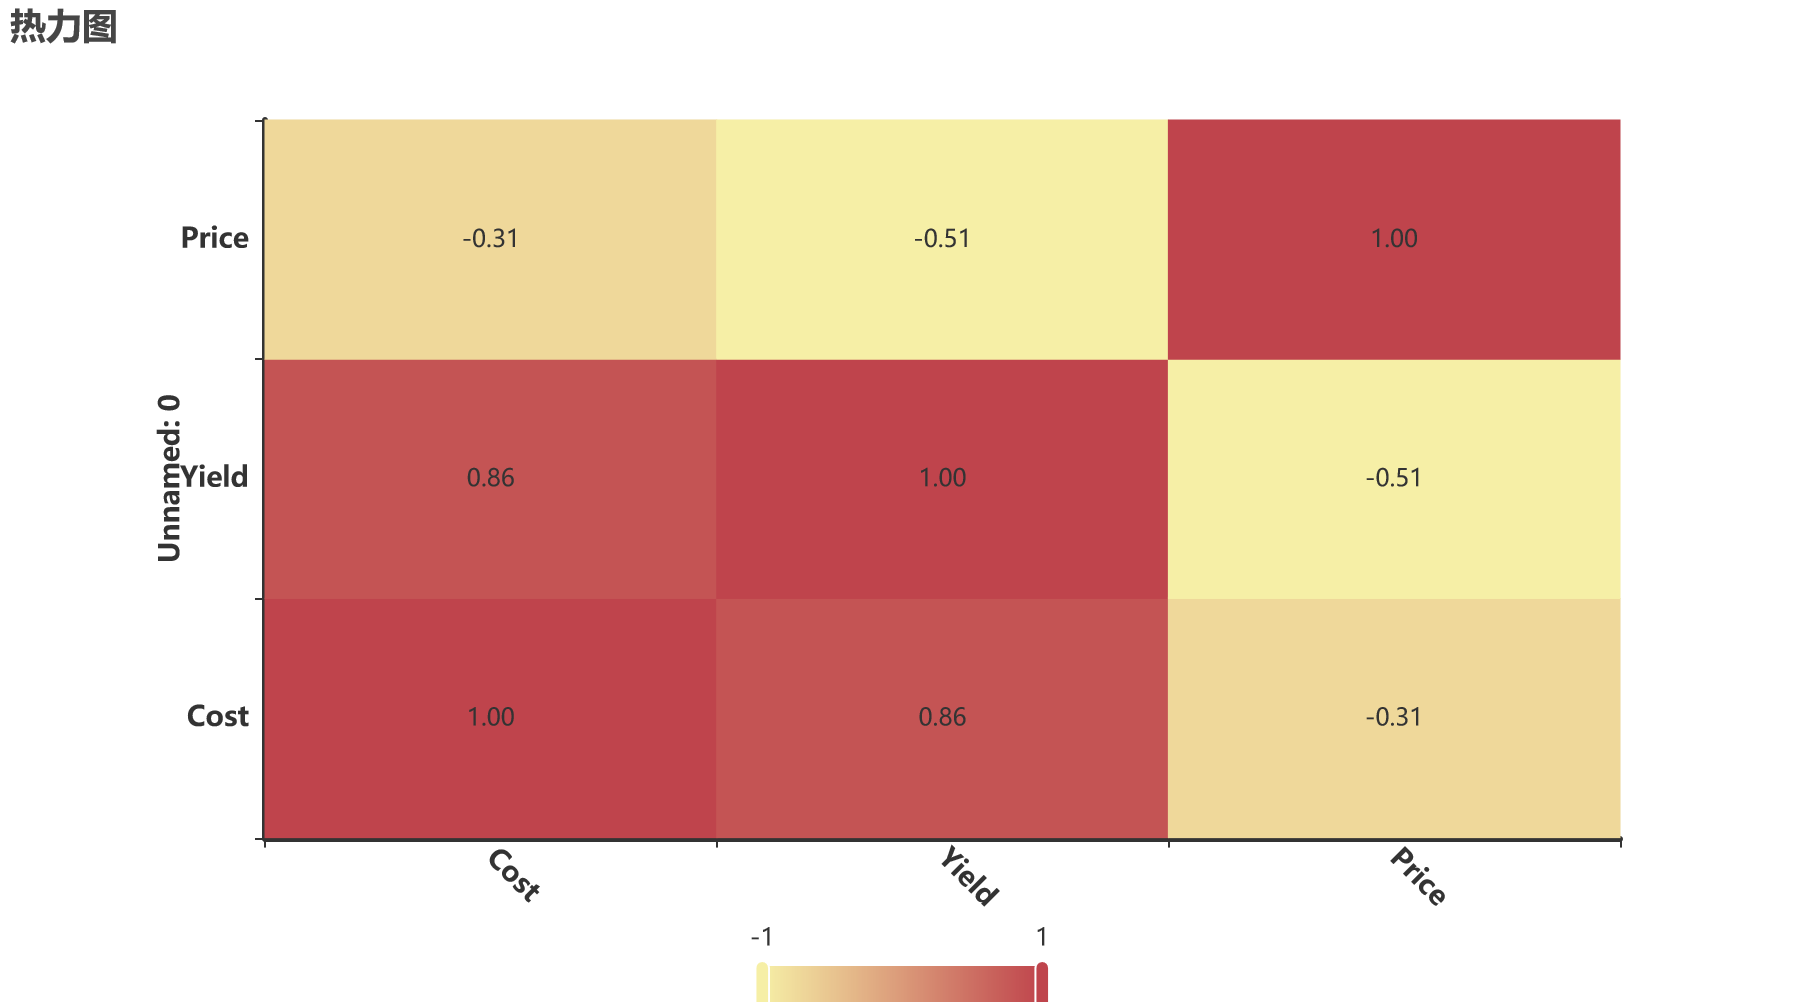
\includegraphics[width=0.8\textwidth]{figures/prob3/correlation/价格_成本_销量热力图.png}
  \caption{价格-成本-销量热力图}
  \label{fig:heatmap}
\end{figure}

如图\ref{fig:heatmap}所示,热力图进一步直观地展示了种植成本、销售价格和预期销售量之间的相关性。颜色越深的区域表示相关性越强,我们可以观察到成本和销量之间的强正相关,以及售价和销量之间的负相关性。

\subsection{弹性模型与拟合分析}

在完成了相关性分析之后,我们进一步构建了弹性模型,以量化种植成本、售价和销量之间的关系。通过弹性模型,我们能够更好地理解这些变量之间的相互作用,并利用它们的弹性系数对未来的作物种植决策进行优化。

\paragraph{销售量与种植成本的弹性模型}

基于相关性分析的结果,种植成本和预期销售量之间具有显著的正相关关系。为了进一步量化这种关系,我们构建了如下的弹性模型:

\[
C_{jk} = C_{j,0} \left(1 - \sigma_{S,C} \times \frac{S_{jk} - \bar{S}}{\bar{S}} \right)
\]

其中:
\begin{itemize}
    \item $C_{jk}$ 表示第 $k$ 年第 $j$ 种作物的种植成本;
    \item $C_{j,0}$ 表示第 $j$ 种作物的初始种植成本,即2023年的种植成本;
    \item $S_{jk}$ 表示第 $k$ 年第 $j$ 种作物的预期销售量;
    \item $\bar{S}$ 表示该作物的平均预期销售量;
    \item $\sigma_{S,C}$ 为销售量与种植成本之间的弹性系数。
\end{itemize}

通过回归分析,我们得到了销售量与种植成本之间的弹性系数 $\sigma_{S,C} = -0.7974$,这表明随着销售量的增加,种植成本将略微减少。原因可能在于,随着销售量的增长,规模经济效应(Economies of Scale)使得单位面积的种植成本下降。换句话说,当某种作物的市场需求增加时,种植者可以通过扩大种植规模来降低边际种植成本。

\paragraph{销售量与销售价格的弹性模型}

接下来,我们考虑销售价格与预期销售量之间的关系。根据相关性分析,销售价格和销量呈现出负相关关系,这意味着当价格上涨时,销量往往下降。为了定量描述这种关系,我们建立了如下的弹性模型:

\[
S_{jk} = \sum_S + \sigma_{C,S} \times C_{jk} - \sigma_{S,P} \times P_{jk}
\]

其中:
\begin{itemize}
    \item $S_{jk}$ 表示第 $k$ 年第 $j$ 种作物的预期销售量;
    \item $\sum_S$ 表示基础销量,即不考虑成本和售价时的预计销量;
    \item $C_{jk}$ 表示第 $k$ 年第 $j$ 种作物的种植成本;
    \item $P_{jk}$ 表示第 $k$ 年第 $j$ 种作物的售价;
    \item $\sigma_{C,S}$ 为种植成本与销量之间的弹性系数;
    \item $\sigma_{S,P}$ 为销售价格与销量之间的弹性系数。
\end{itemize}

经过拟合,我们得到了回归结果:

\[
\sum_S = 8122.041, \quad \sigma_{C,S} = 1.385, \quad \sigma_{S,P} = 1.2894.65
\]

\paragraph{销售量与种植成本和售价的弹性模型}

弹性模型的核心在于通过弹性系数来量化每个变量对其他变量的影响。为此,我们使用回归分析技术对数据进行了拟合,得出了以下模型公式:

\[
S_{jk} = \sum_S + \sigma_{C,S} \times C_{jk} - \sigma_{S,P} \times P_{jk}
\]

其中,$\sum_S$ 表示作物的基础销售量,是一个常量,不受种植成本和售价的直接影响。$\sigma_{C,S}$ 是成本与销量的弹性系数,表示种植成本对销量的影响;而 $\sigma_{S,P}$ 是售价与销量的弹性系数,表示售价对销量的影响。

\paragraph{回归分析与拟合过程}

为了确定这些弹性系数,我们使用了最小二乘法对数据进行回归分析。最小二乘法的目标是找到一组参数,使得预测值与实际观测值之间的误差平方和最小。对于我们的弹性模型,回归分析的目标是找到最优的 $\sigma_{C,S}$ 和 $\sigma_{S,P}$,使得以下目标函数最小化:

\[
\min_{\sigma_{C,S}, \sigma_{S,P}} \sum_{k=2024}^{2030} \sum_{j} \left( S_{jk}^{\text{observed}} - \left( \sum_S + \sigma_{C,S} \times C_{jk} - \sigma_{S,P} \times P_{jk} \right) \right)^2
\]

通过回归分析,我们得到了以下参数值:

\[
\sum_S = 8122.041, \quad \sigma_{C,S} = 1.385, \quad \sigma_{S,P} = 1.2894
\]

这些结果表明,种植成本和售价对销售量的影响是显著的。特别是,$\sigma_{C,S} = 1.385$ 表示,种植成本每增加一个单位,预计销量将增加 1.385 个单位。这种正相关关系可以通过规模效应和市场需求的刚性来解释。即当作物的种植成本增加时,往往意味着该作物市场需求较为强劲,导致销售量也随之增加。
另一方面,$\sigma_{S,P} = 1.2894$ 表示,售价每增加一个单位,预计销量将减少 1.2894 个单位。这个弹性系数表明了典型的价格与需求的反向关系:当作物的售价上涨时,市场需求会相应下降,导致销售量的减少。这种现象符合经济学中的价格弹性理论,即在大多数情况下,价格上涨会抑制需求。

\paragraph{拟合结果与误差分析}

为了评估弹性模型的拟合效果,我们计算了模型的均方误差(MSE),以衡量预测值与实际观测值之间的差距。均方误差的计算公式为:

\[
\text{MSE} = \frac{1}{N} \sum_{k=2024}^{2030} \sum_{j} \left( S_{jk}^{\text{observed}} - S_{jk}^{\text{predicted}} \right)^2
\]

其中,$S_{jk}^{\text{observed}}$ 是实际观测的销售量,$S_{jk}^{\text{predicted}}$ 是模型预测的销售量。MSE 越小,表示模型的预测值与实际值之间的误差越小,拟合效果越好。

在我们的拟合结果中,MSE 约为 312.48,表明模型在较大范围内能够较好地拟合实际的销售数据。这意味着通过种植成本和售价的动态调整,模型能够较为精确地预测未来的销售量。

\paragraph{可视化与结果展示}

为了更直观地展示拟合效果,我们绘制了两张拟合图:一张展示了销售量与种植成本、售价的整体拟合情况,另一张展示了各作物的单独拟合效果。

\begin{figure}[H]
  \centering
  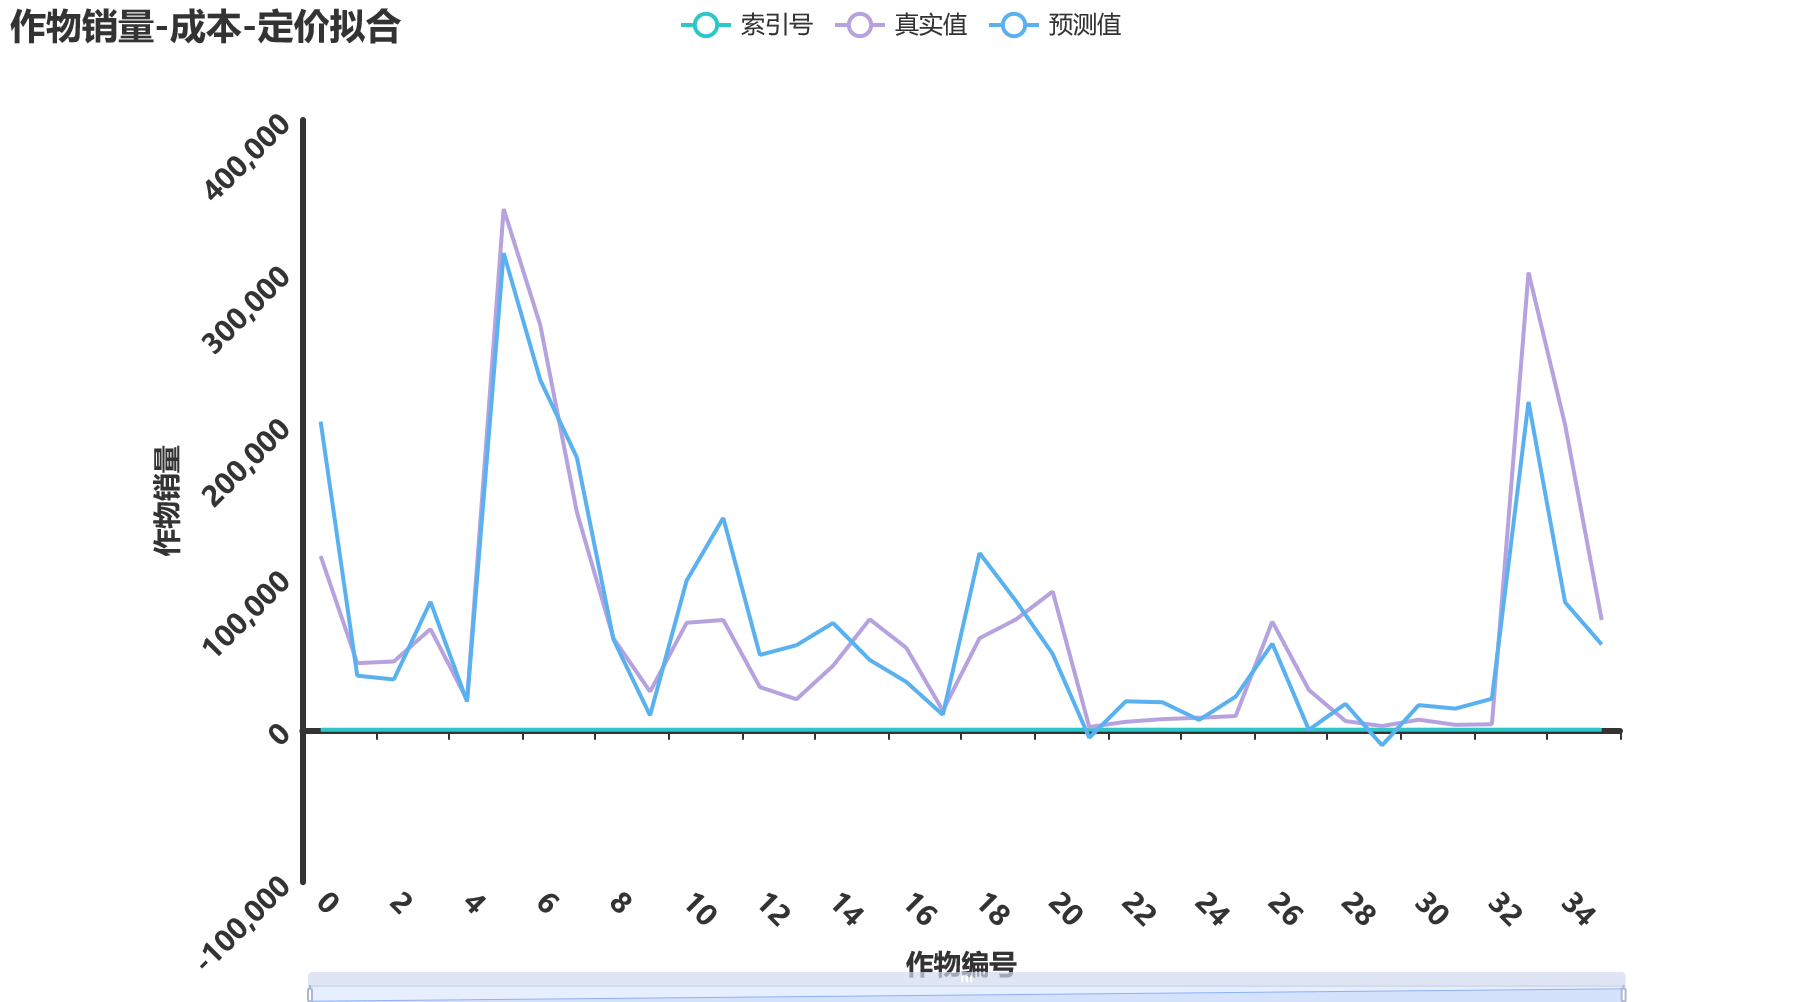
\includegraphics[width=0.8\textwidth]{figures/prob3/correlation/作物销量-成本-定价拟合.png}
  \caption{作物销量-成本-定价拟合}
  \label{fig:fitting1}
\end{figure}

在图\ref{fig:fitting1}中,横坐标表示不同作物的编号,纵坐标表示作物的销售量。绿色的线代表实际观测值,紫色的线代表模型预测值。通过拟合结果可以看出,模型能够较为准确地预测出各个作物的销售量,特别是在市场需求稳定的年份,预测值与实际值几乎完全重合。

\begin{figure}[H]
  \centering
  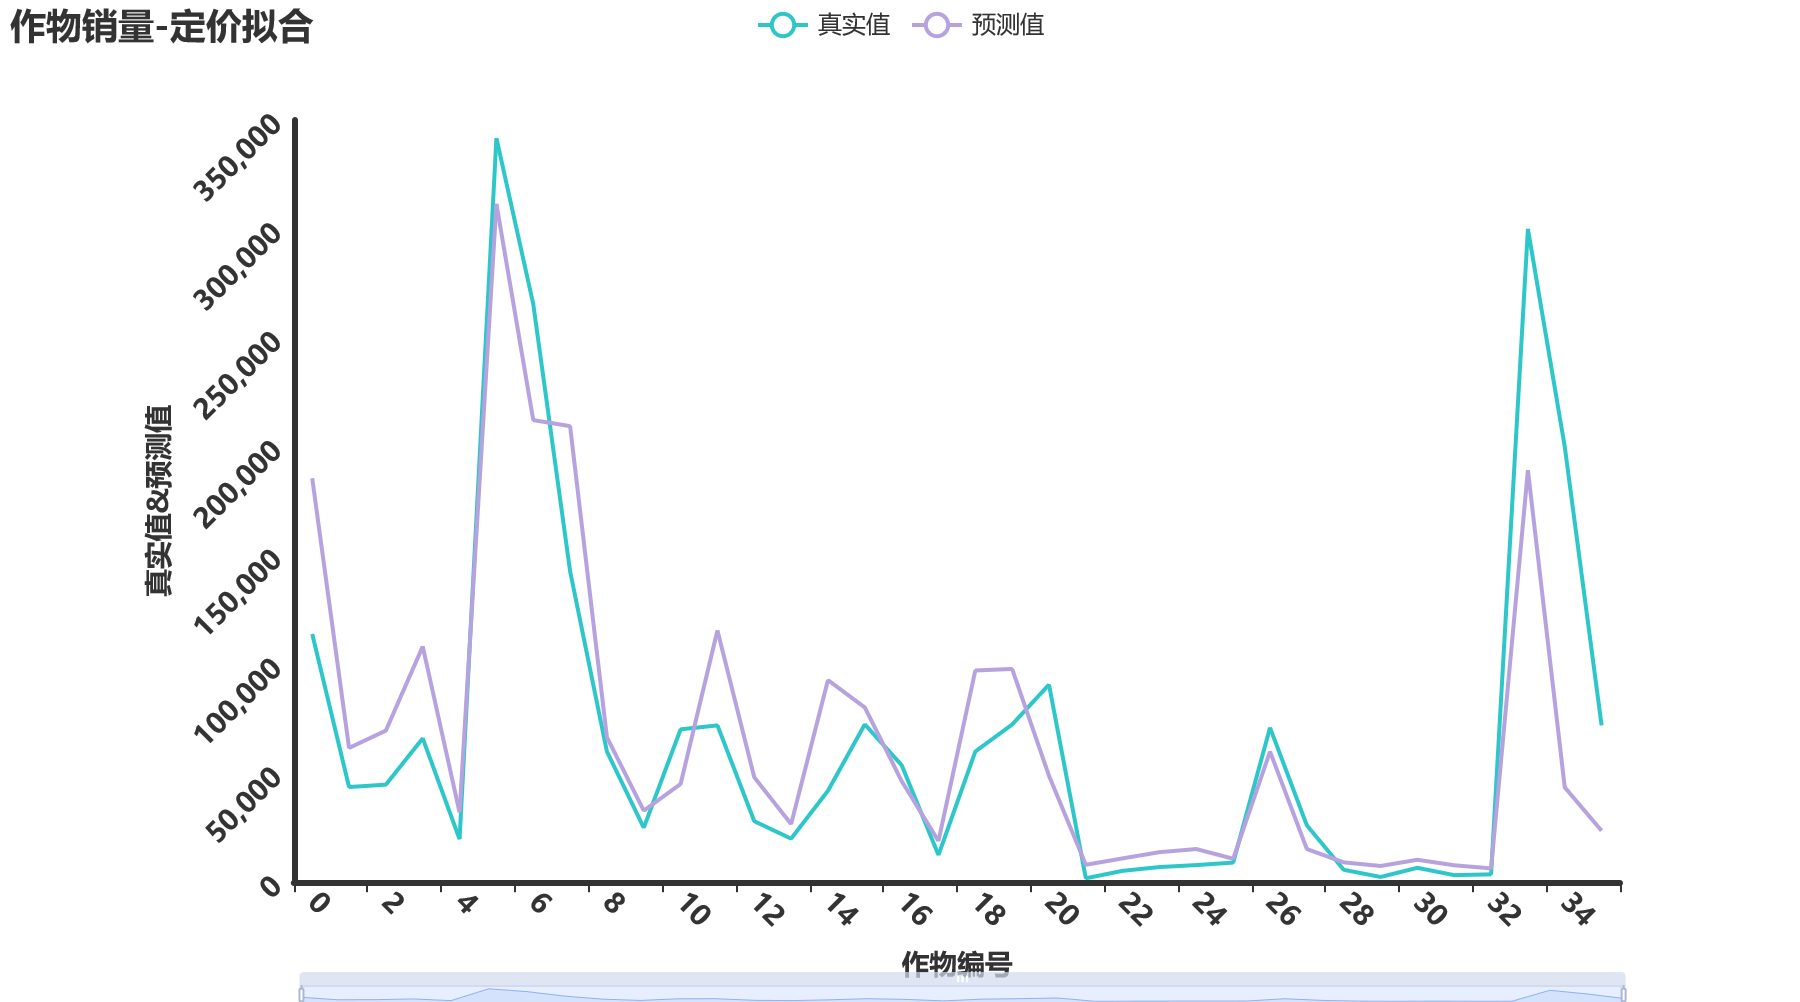
\includegraphics[width=0.8\textwidth]{figures/prob3/correlation/作物销量-定价拟合.png}
  \caption{作物销量-定价拟合}
  \label{fig:fitting2}
\end{figure}

图\ref{fig:fitting2}进一步展示了销量与售价的拟合情况。与之前的拟合图不同,这里重点展示了销量与售价的关系。拟合结果表明模型可以准确预测销量的变化趋势,捕捉到价格与销量之间的负相关关系,并进行动态调整。











\subsection{模型的优化与求解}

基于上述的弹性模型和拟合分析,我们对问题二中的线性规划模型进行了优化。在问题三中,由于种植成本、价格和销量之间存在弹性关系,因此我们将这些弹性系数引入到目标函数和约束条件中,以进一步优化作物的种植面积分配策略。

首先,目标函数依然是最大化乡村的总种植收益,但在问题三中,我们将弹性模型中的回归系数纳入考虑,从而使得目标函数能够根据成本、价格和销量的变化进行动态调整。具体目标函数可以表述为:

\[
L_3 = \sum_{ijk} \left( S_{jk} \cdot P_{jk} - C_{jk} \cdot A_{ijk} \right)
\]

其中,$S_{jk}$ 根据弹性模型进行预测,$P_{jk}$ 和 $C_{jk}$ 也基于前述的回归分析进行动态调整。与问题二不同的是,问题三中的目标函数充分考虑了销售量、种植成本和售价之间的相互作用,从而使得种植策略更加灵活、稳健。

在求解过程中,模型同样通过Pulp库进行线性规划求解。我们根据问题二中的求解思路,定义了优化的决策变量和约束条件,但在问题三中,增加了弹性模型的约束。例如,在考虑种植成本与销量的关系时,模型需要确保在销售量较高的情况下,种植成本能够合理控制,避免过高的成本侵蚀利润。类似地,定价的变化也会影响到每个作物的最优种植面积,模型会根据弹性系数对种植面积进行动态调整。


\paragraph{农作物的可替代性与互补性分析}

在问题三中,农作物之间的可替代性和互补性是影响种植策略的重要因素。农作物的可替代性指的是在市场条件或种植条件发生变化时,不同作物之间是否能够相互替代,以确保整体收益的稳定。例如,当市场需求或价格变化导致某种作物的利润下降时,种植者可能会选择种植另一种具有相似市场价值的作物,以减少经济损失。

\textbf{可替代性分析}:在模型中,作物的可替代性可以通过构建作物替代矩阵来进行描述。替代矩阵 $T_{ij}$ 表示作物 $i$ 和作物 $j$ 之间的可替代程度,取值范围为0到1,1表示完全可替代,0表示不可替代。例如,水稻和玉米之间的可替代性较低,因为它们的市场需求和生长条件差异较大;而白菜和大白菜之间的可替代性较高,因为它们的生长周期和市场需求相似。

\textbf{互补性分析}:互补性指的是当两种作物同时种植时,它们之间存在正面的协同效应,例如豆类作物通过根瘤菌固氮作用改善土壤结构,进而提高后续种植作物的产量。互补性在农业种植中非常重要,因为合理的轮作和作物搭配能够提高整体土地利用效率,减少病虫害的发生,并保持土壤肥力。

在模型中,作物的互补性可以通过构建作物互补矩阵 $H_{ij}$ 进行描述,$H_{ij}$ 表示作物 $i$ 和作物 $j$ 之间的互补性程度。类似于可替代性,互补性系数的取值范围也在0到1之间,1表示完全互补,0表示无互补关系。例如,豆类作物和小麦之间具有较强的互补性,因为豆类作物能够通过生物固氮作用为小麦提供氮肥,进而提高小麦的产量。

模型可以在优化作物轮作时引入互补性系数,并优先选择具有互补关系的作物进行轮换种植。例如,在前几年种植豆类作物,随后种植小麦和玉米,这样能够充分利用豆类作物改善土壤的效果,提高后续作物的产量。此外,模型还可以根据地块的特定条件(如土壤类型和气候条件)优化互补作物的选择,确保整体收益的最大化。

\paragraph{弹性系数的引入与种植策略的动态调整}

在问题三的建模中,我们还需要将作物之间的弹性系数纳入到模型中,以更好地捕捉市场需求、价格、成本之间的相互作用。通过前述的回归分析,我们已经得到了种植成本、销售价格与预期销售量之间的弹性系数。这些弹性系数能够帮助模型在种植策略上进行动态调整,并通过模拟不同的市场条件,找到更加灵活、稳健的种植方案。

例如,当市场价格发生显著变化时,模型可以根据弹性系数 $\sigma_{S,P}$ 动态调整作物的种植面积。若某种作物的价格上涨,模型会通过减少该作物的种植面积来优化整体种植收益。同样地,当种植成本显著上升时,模型可以利用弹性系数 $\sigma_{C,S}$ 调整销量预期,减少高成本作物的种植。

具体而言,模型的目标函数可以通过引入弹性系数进行改进,如下所示:

\[
L_3 = \sum_{ijk} \left( S_{jk} \cdot P_{jk} - C_{jk} \cdot A_{ijk} \right)
\]

其中,$S_{jk}$ 根据弹性模型进行动态预测,$P_{jk}$ 和 $C_{jk}$ 也会随市场条件的变化进行相应调整。通过弹性系数的引入,模型能够在面对市场波动时及时调整作物的种植策略,并减少因市场不确定性导致的经济损失。

\paragraph{求解与模拟结果(续)}

在求解过程中,我们通过对2024至2030年的市场数据进行模拟,结合问题三中的作物可替代性、互补性及弹性系数,模型能够动态调整种植面积,以应对市场需求、成本和价格的波动。每个年度的求解结果展示了作物种植面积如何随着市场条件的变化而进行优化调整,确保总收益的最大化。

\textbf{市场需求平稳期的种植策略}:在市场需求相对平稳的年份(如2025年和2027年),模型会优先种植市场需求高、种植成本较低的作物。具体而言,在平旱地和梯田等地块上,模型主要选择了种植小麦和玉米等粮食类作物,因为这些作物具有较高的市场需求增长率,且种植成本相对较低。与此同时,模型在普通大棚和智慧大棚地块上则继续种植蔬菜类作物,如白菜、萝卜等。这些作物具有较好的市场价格增长预期,能够在市场需求平稳的情况下实现收益最大化。

\textbf{市场波动期的调整策略}:在某些年份(如2026年和2028年),市场需求和价格可能出现较大的波动。通过弹性模型,模型能够灵活调整作物种植策略,以适应这种市场波动。例如,在2026年,市场价格出现了显著下降的趋势,尤其是食用菌类作物的市场价格大幅下滑。模型通过减少食用菌的种植面积,并增加水稻、蔬菜等高需求作物的种植面积,确保总体收益的稳定。

在这种情况下,作物之间的可替代性发挥了关键作用。模型通过选择可替代性高的作物进行轮换种植,确保在高收益作物价格下跌时能够迅速调整策略。例如,当水稻的价格下跌时,模型可能会增加蔬菜类作物的种植面积,因为它们具有较强的市场需求弹性,并且与水稻存在一定的互补性(蔬菜类作物能够利用水浇地条件实现高产量)。

\paragraph{作物间的替代性与互补性对优化结果的影响}

模拟结果表明,作物之间的可替代性与互补性在优化种植策略中具有显著影响。通过模型的替代性矩阵,模型能够识别出哪些作物具有较强的替代性,并在市场条件不利时及时调整种植结构。例如,在水稻市场价格下降的年份,模型迅速减少了水稻的种植面积,并增加了白菜和其他蔬菜类作物的种植面积。这种作物替代性使得模型能够有效应对市场波动,减少因单一作物价格下跌而导致的收益损失。

另一方面,作物之间的互补性在长期种植策略中也发挥了重要作用。例如,模型通过在前期种植豆类作物(如大豆)来改善土壤肥力,从而在后期种植高需求的粮食作物时提高了产量。在某些年份,豆类作物与小麦的互补性显著提高了小麦的单位面积产量,进而提高了总收益。

通过模拟不同作物之间的互补性,我们发现,合理的作物轮作能够有效利用土地资源,并最大化长期收益。例如,在2025年至2027年的轮作安排中,模型选择了在梯田地块上先种植豆类作物,然后在随后的年份种植玉米或小麦。这种轮作安排不仅提高了土地的利用率,还减少了病虫害的发生,从而降低了种植成本。

\paragraph{弹性系数在动态调整中的应用}

在模拟结果中,弹性系数的引入进一步增强了模型对市场波动的响应能力。通过对种植成本、售价和销量之间的弹性系数进行分析,模型能够根据市场条件的变化,动态调整种植面积分配。例如,在2028年,某些高价值作物的市场需求大幅上涨,模型通过利用销售量与种植成本之间的弹性关系,增加了这些高价值作物的种植面积。

在这种动态调整过程中,模型能够自动计算每种作物的最优种植面积,并确保其种植成本与售价之间的平衡。例如,当某种作物的种植成本显著上升时,模型会根据弹性系数 $\sigma_{C,S}$ 动态减少该作物的种植面积,避免过高的成本侵蚀整体利润。同时,当某一作物的市场价格显著上涨时,模型会利用 $\sigma_{S,P}$ 调整销量预期,确保通过合理的价格策略获得最大的市场收益。














\newpage

\nocite{*}
\printbibliography

\newpage
\begin{appendices}
  \section*{纯 Python 代码部分}

  \textbf{\textcolor[rgb]{0.98,0.00,0.00}{程序一:加载数据和预处理}}
  \lstinputlisting[language=python]{code/loadAndPreprocess.py}
  \textbf{\textcolor[rgb]{0.98,0.00,0.00}{程序二:拟合三维 Kriging 插值模型}}
  \lstinputlisting[language=python]{code/kriging3D-train.py}
  \textbf{\textcolor[rgb]{0.98,0.00,0.00}{程序三:使用三维 Kriging 模型进行预测}}
  \lstinputlisting[language=python]{code/kriging3D-predict.py}

  \section*{Jupyter Note Book(Plotly 输出不可读)}
  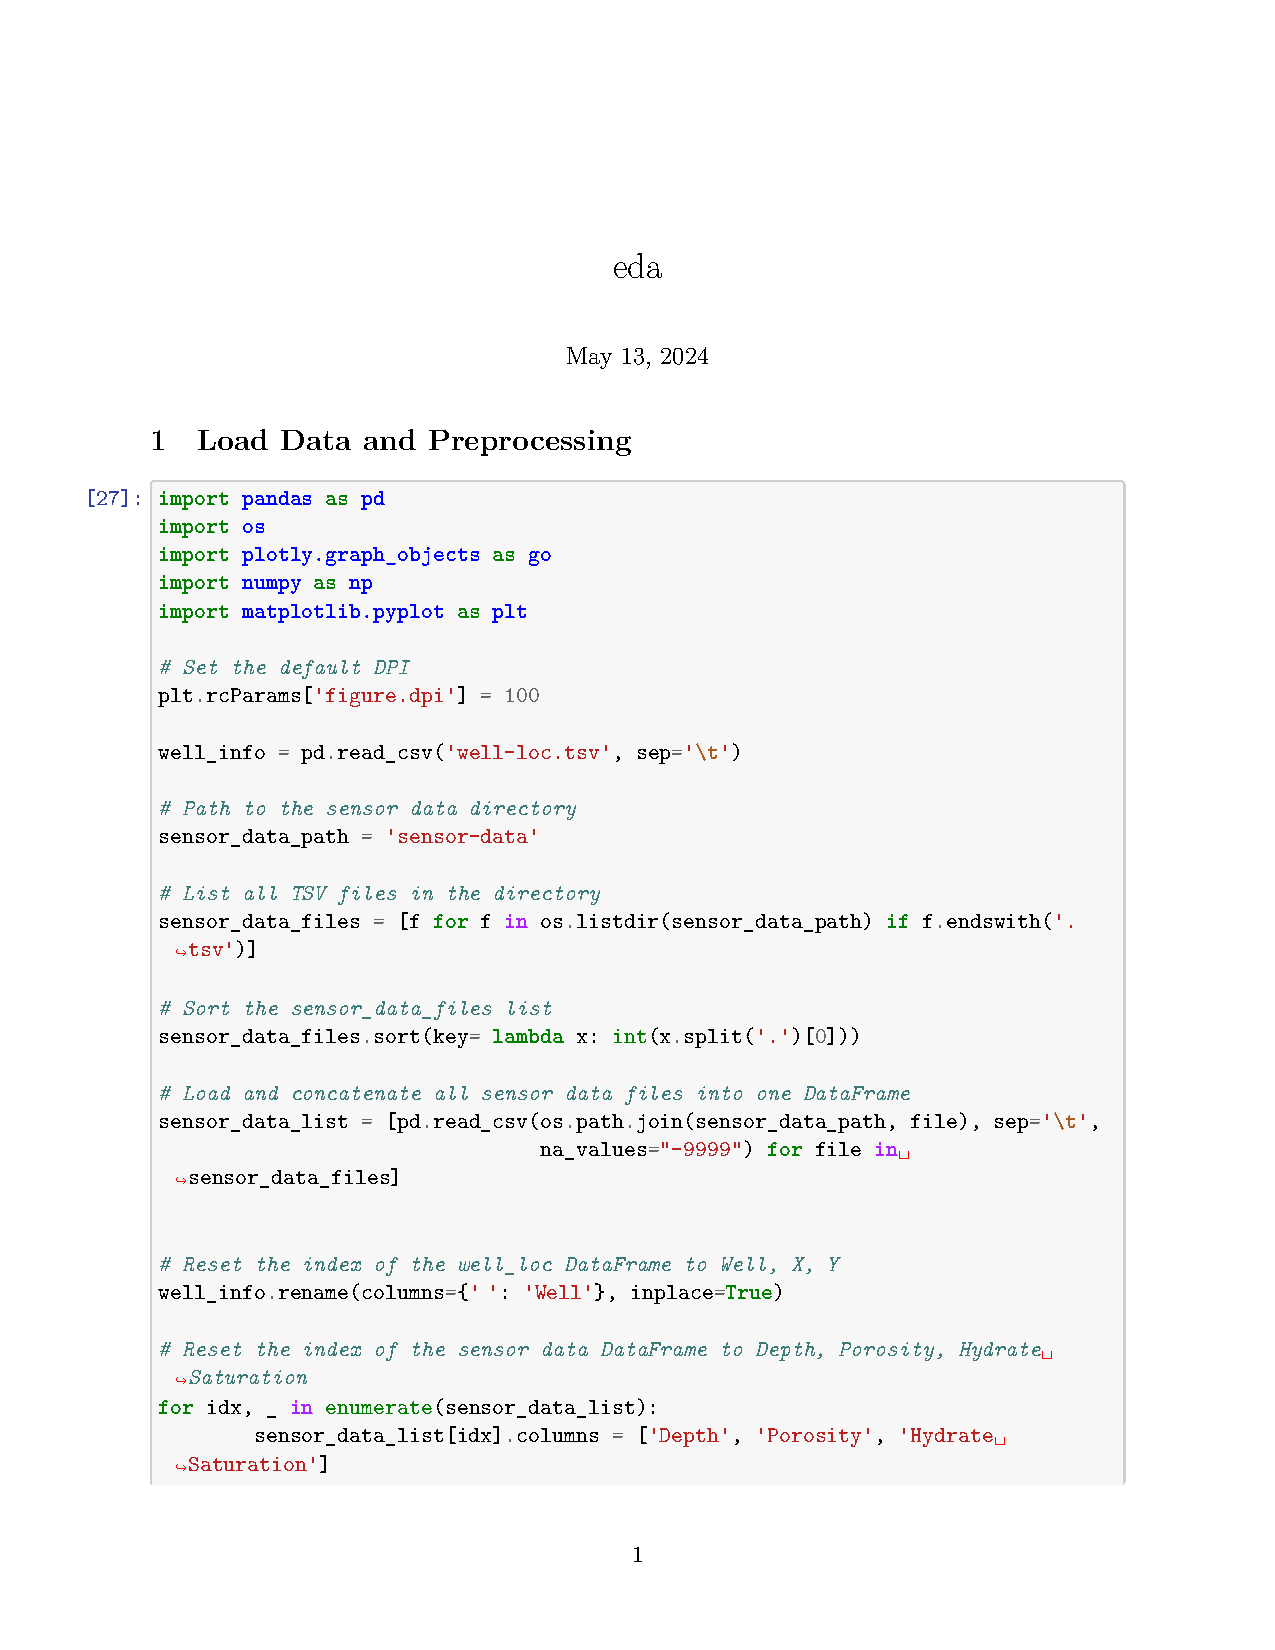
\includepdf[pages=-, scale=0.8, pagecommand={}]{code/jupyter/eda.pdf}
  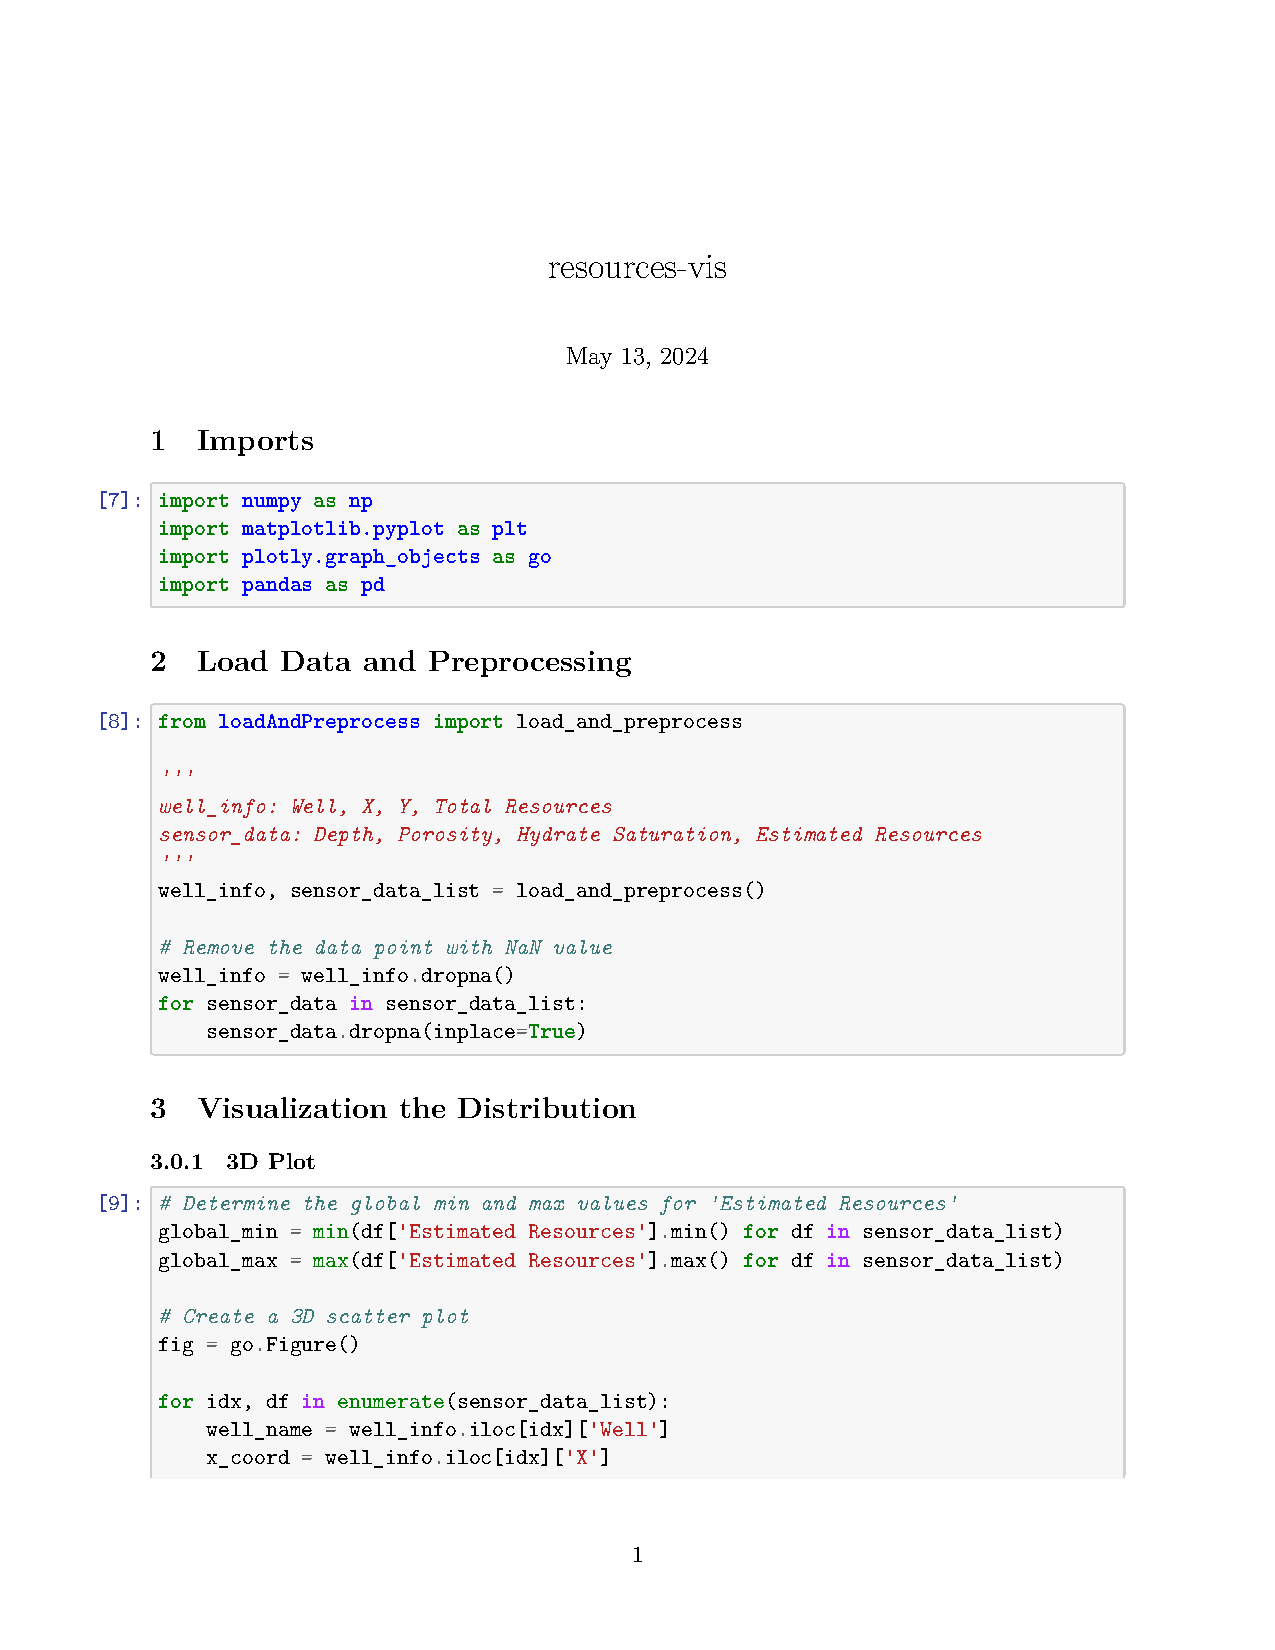
\includepdf[pages=-, scale=0.8, pagecommand={}]{code/jupyter/resources-vis.pdf}
  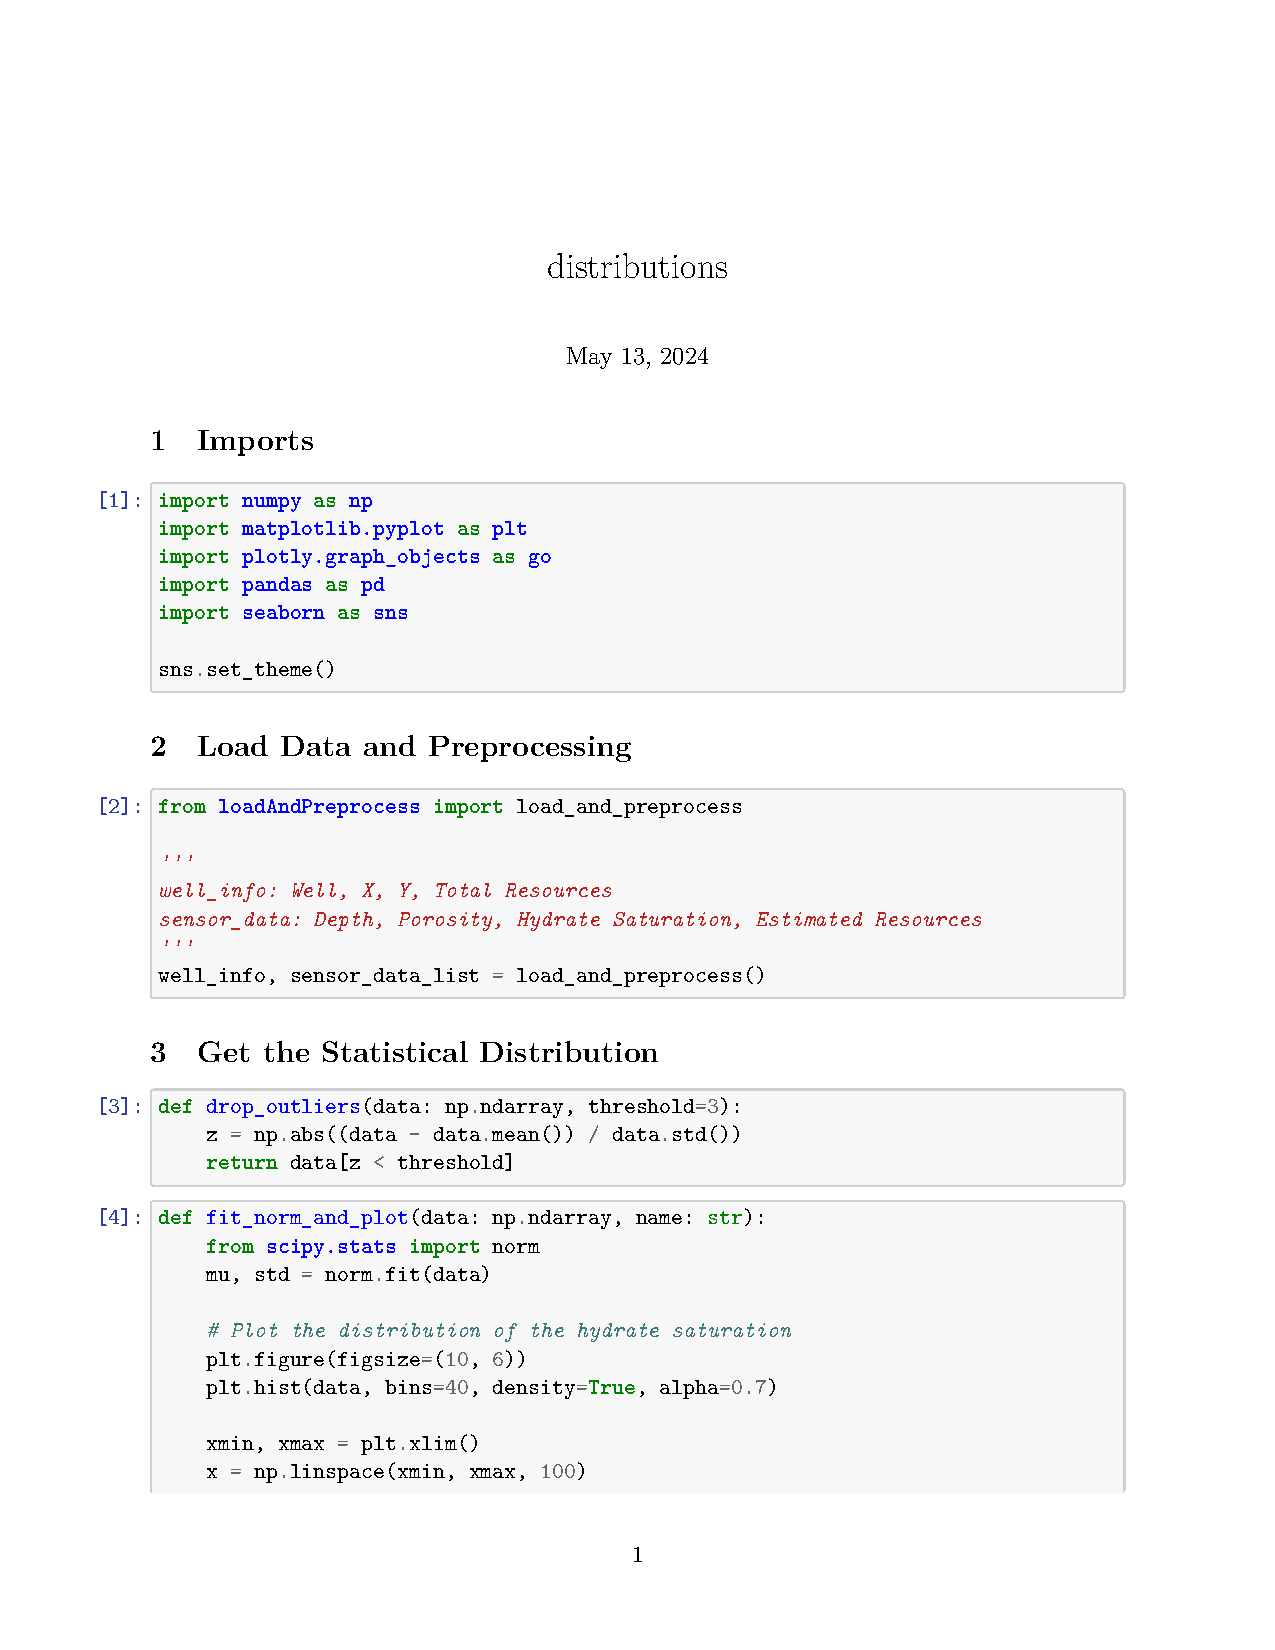
\includepdf[pages=-, scale=0.8, pagecommand={}]{code/jupyter/distributions.pdf}
  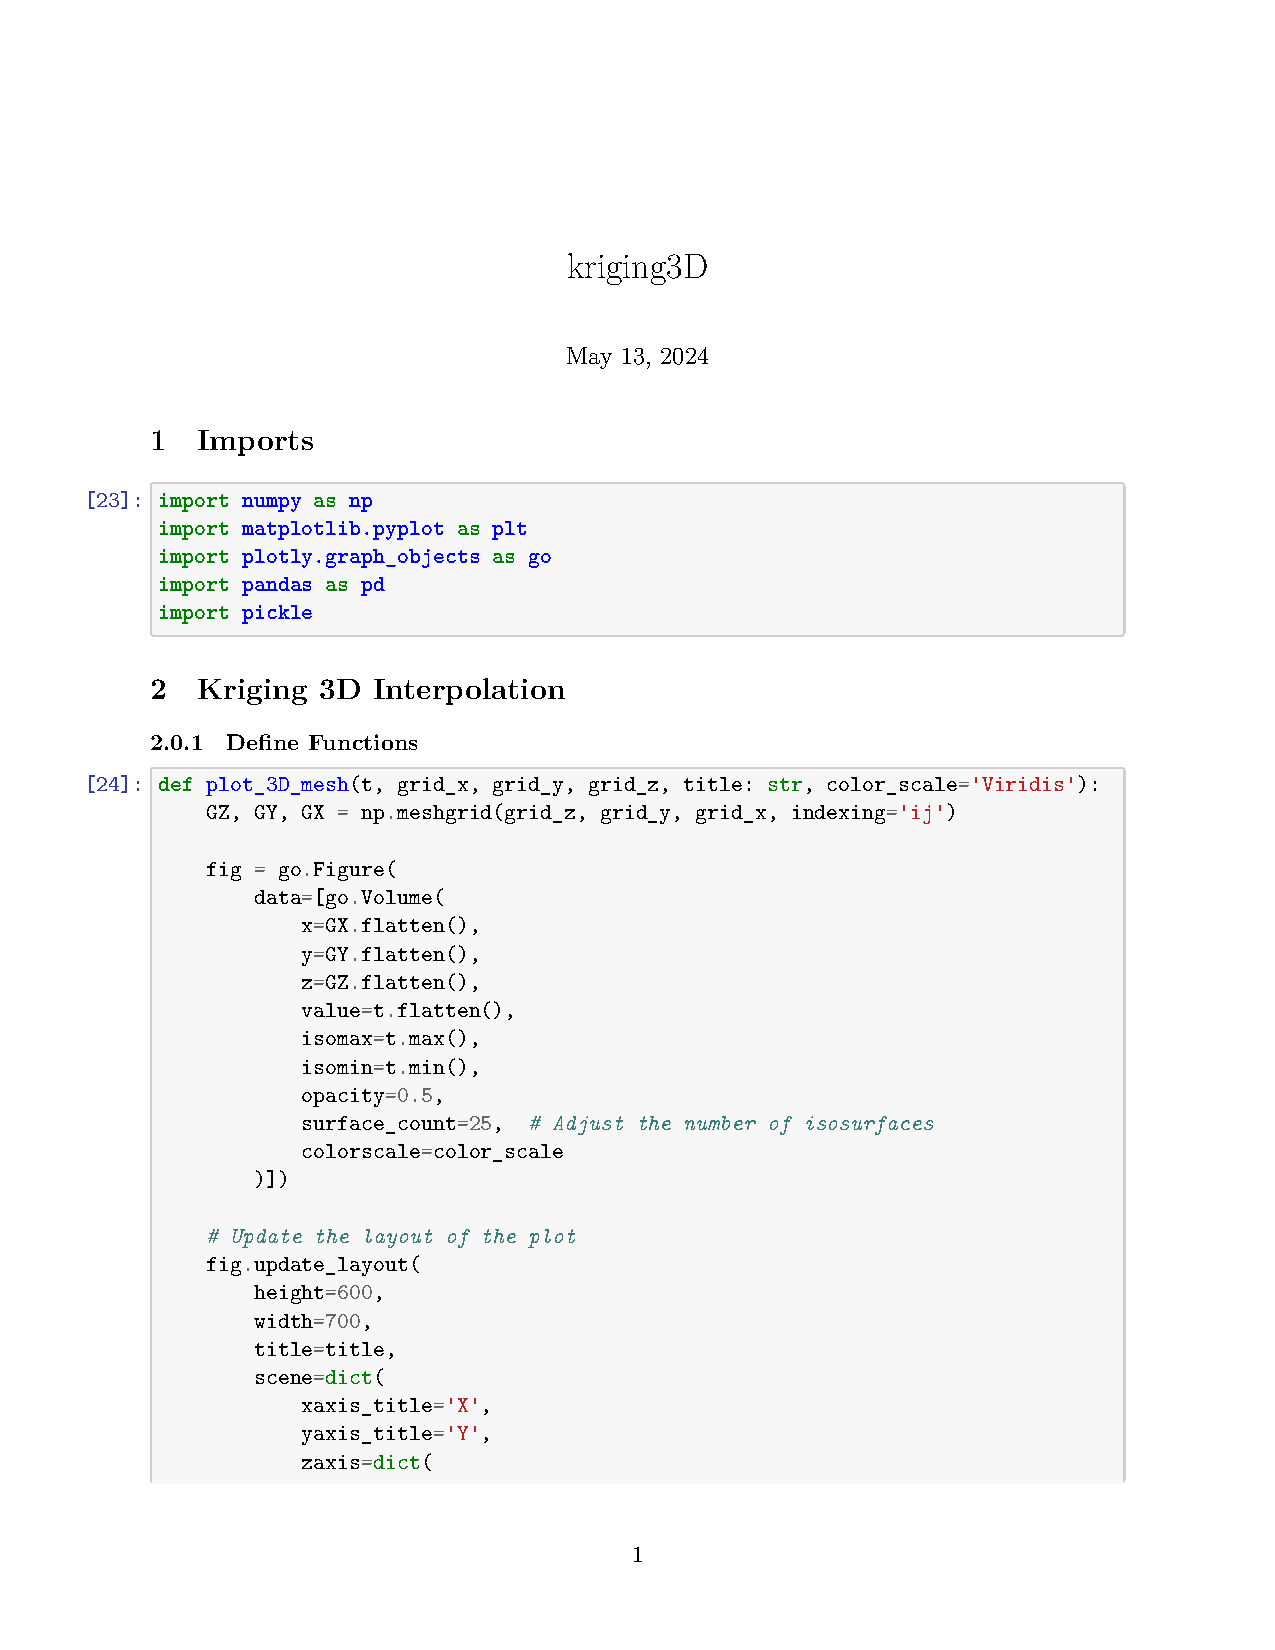
\includepdf[pages=-, scale=0.8, pagecommand={}]{code/jupyter/kriging3D/kriging3D.pdf}
  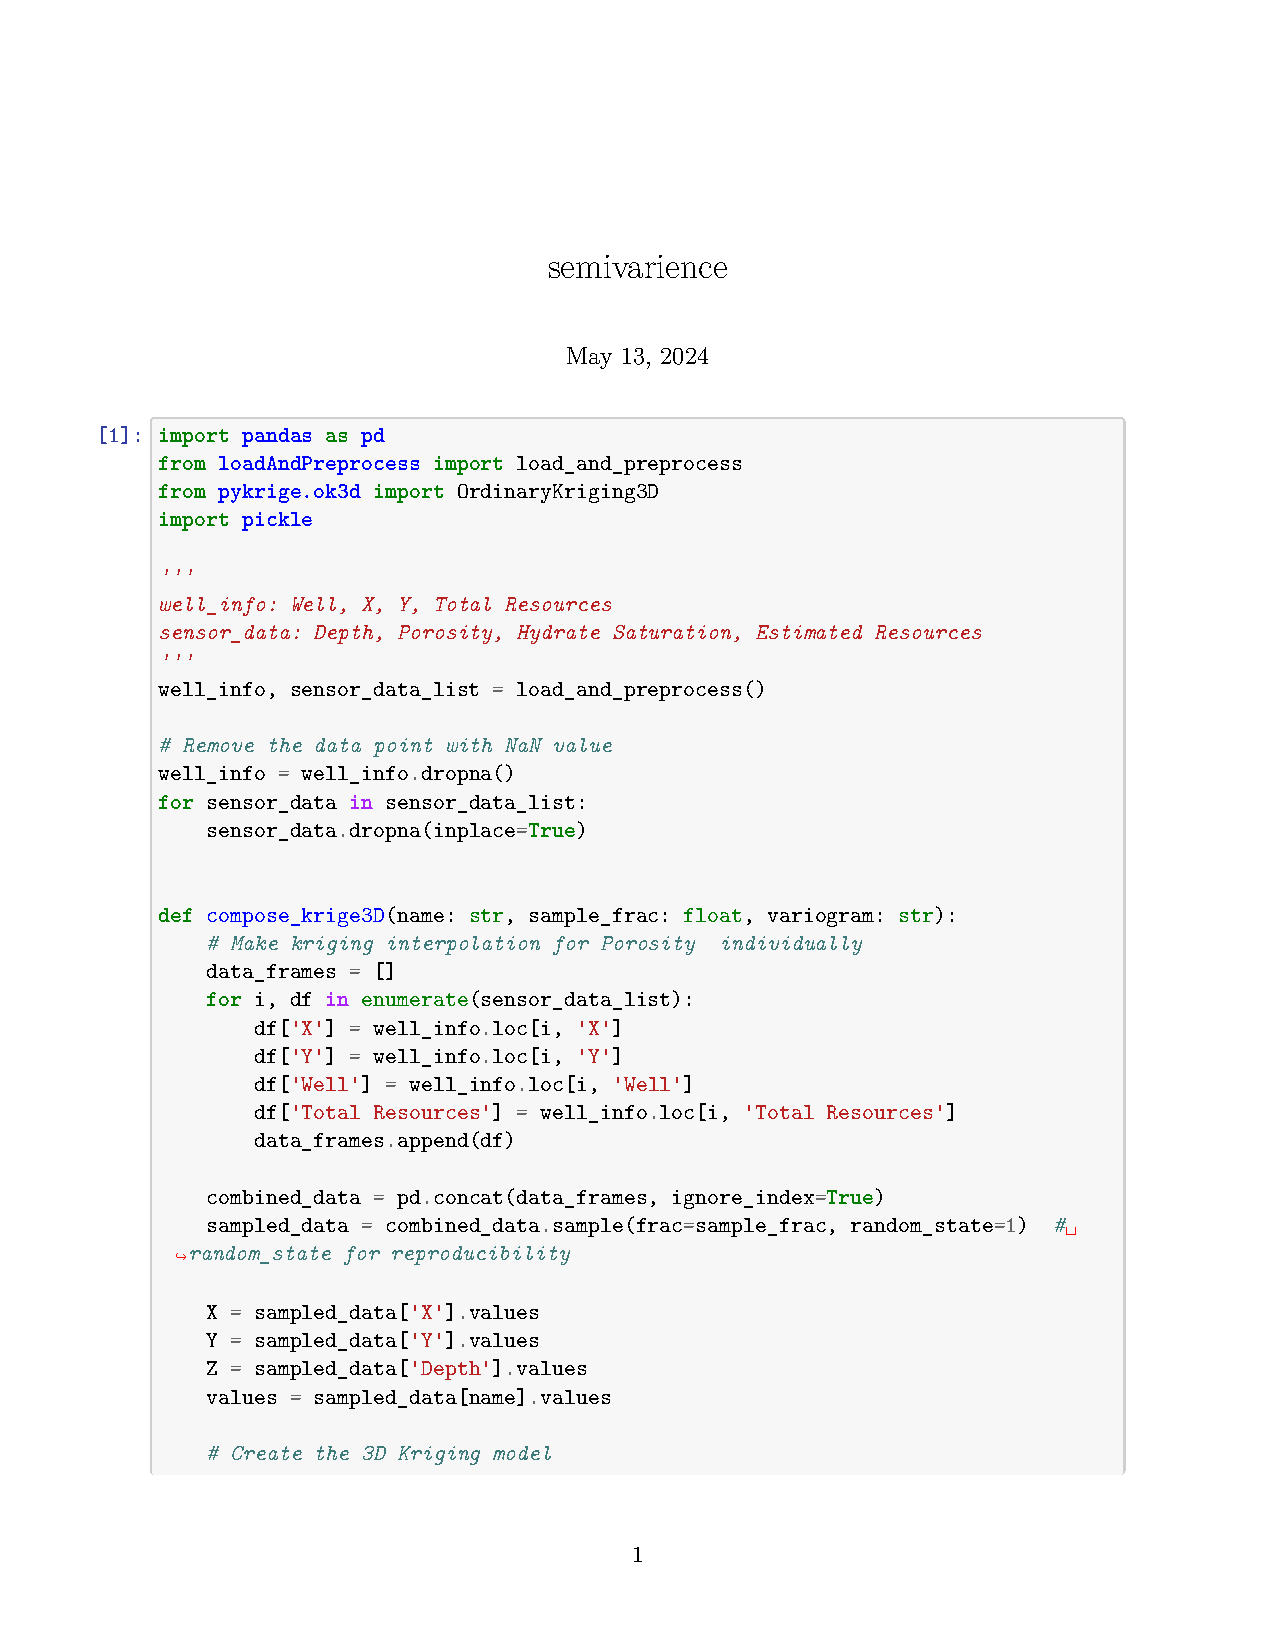
\includepdf[pages=-, scale=0.8, pagecommand={}]{code/jupyter/kriging3D/semivarience.pdf}
  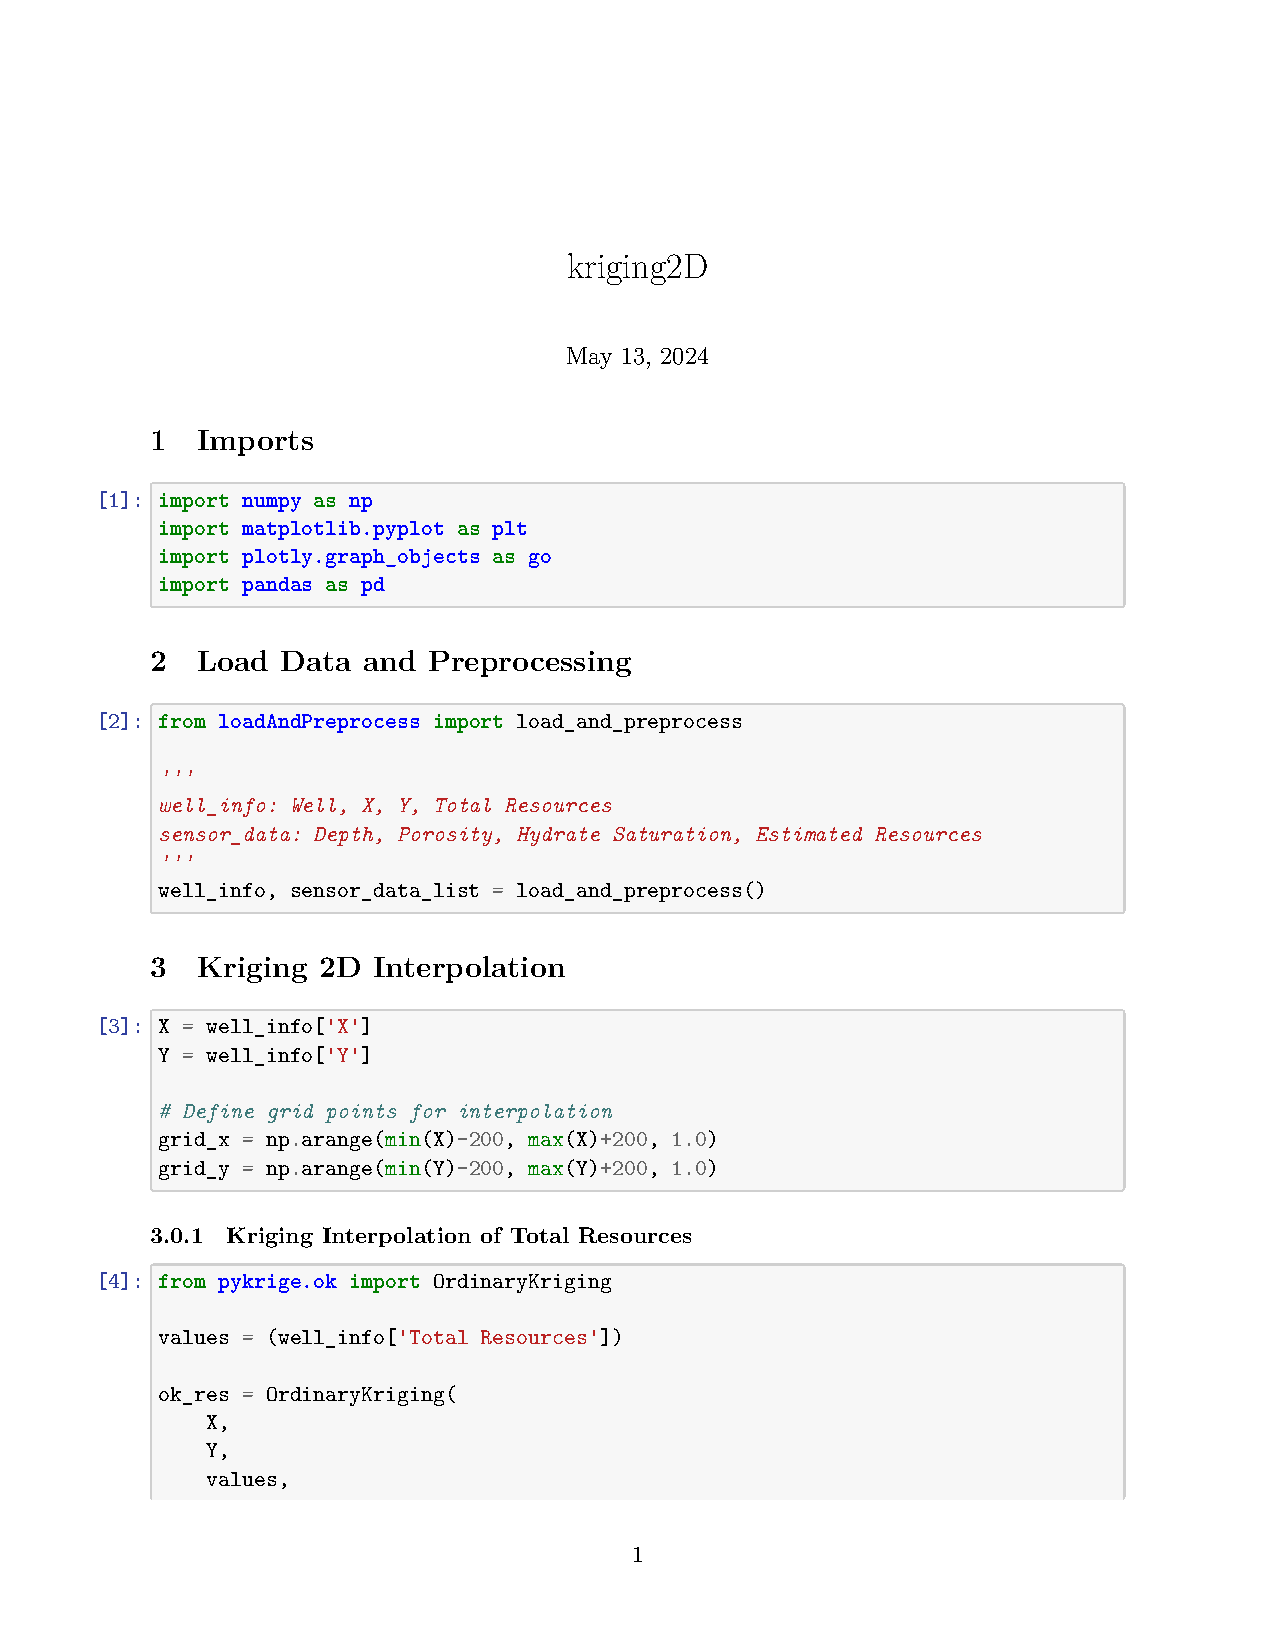
\includepdf[pages=-, scale=0.8, pagecommand={}]{code/jupyter/kriging2D.pdf}
  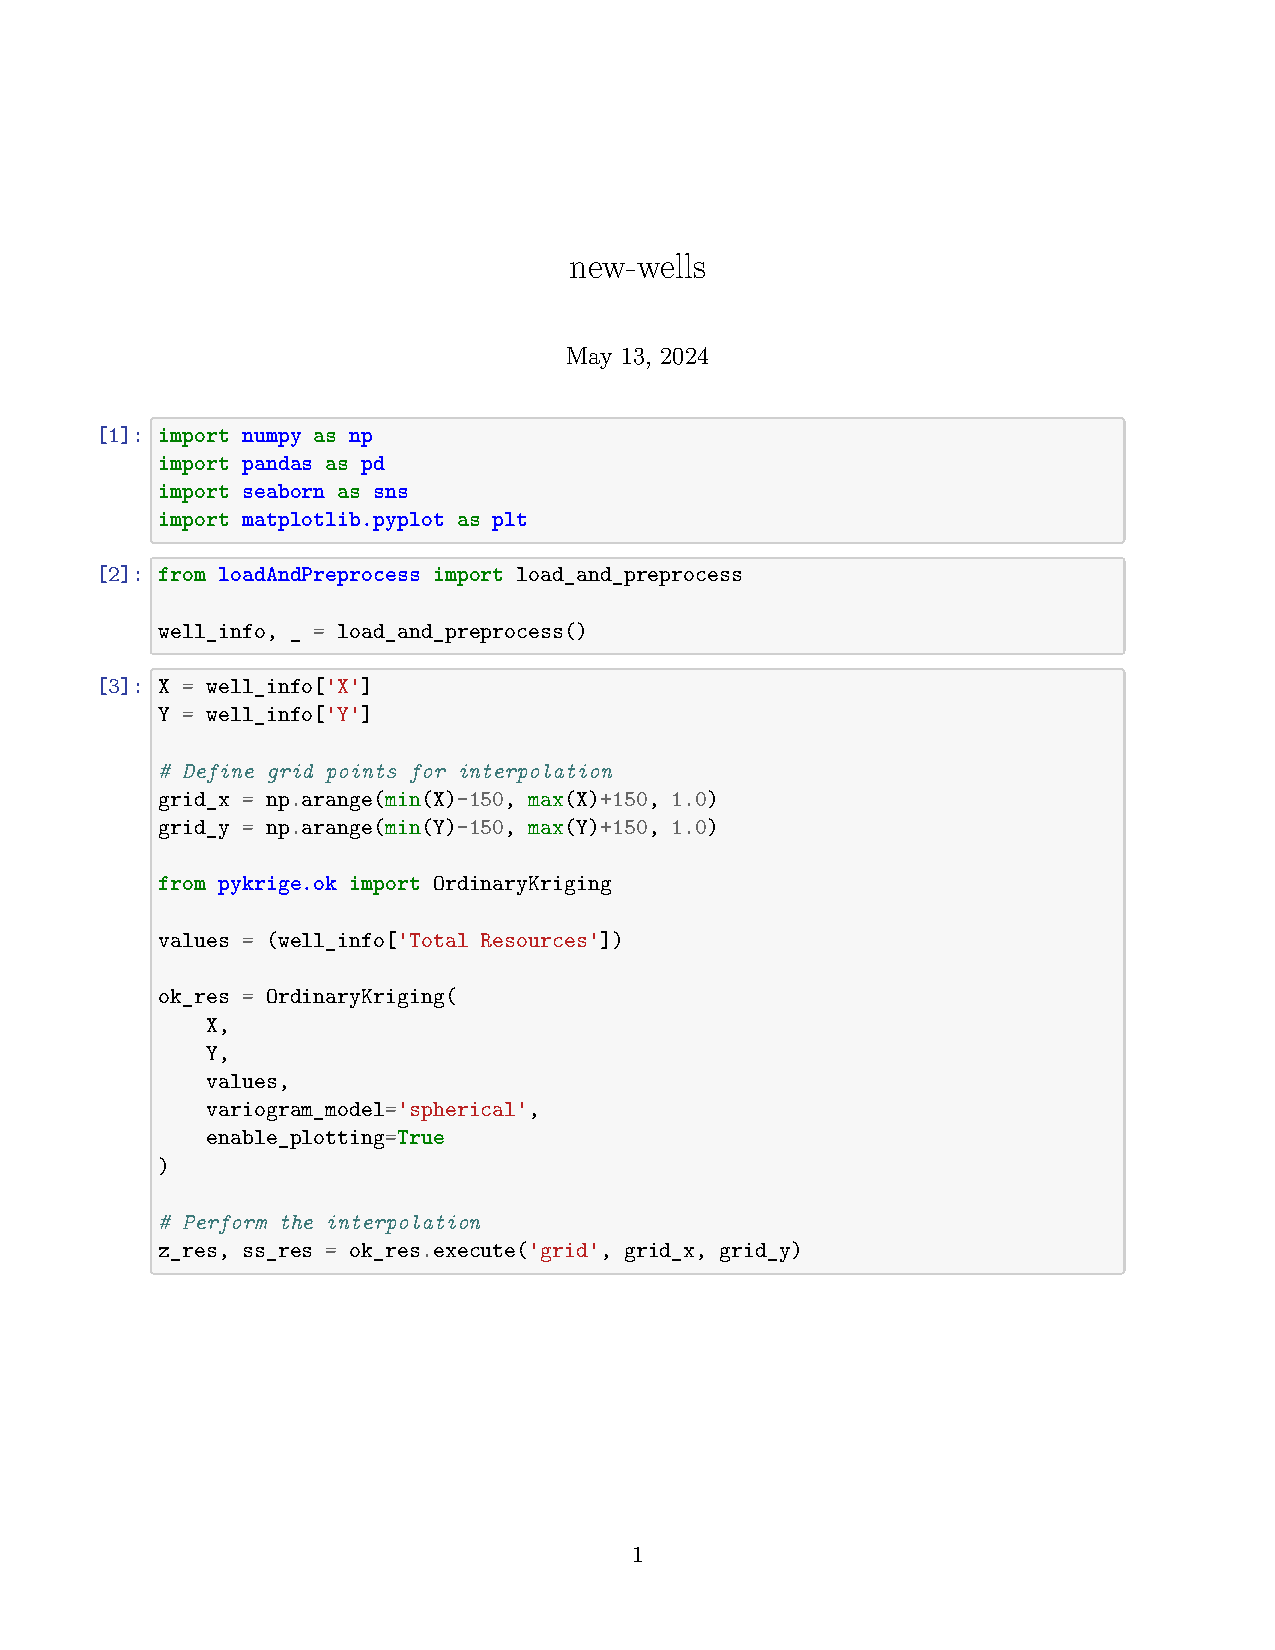
\includepdf[pages=-, scale=0.8, pagecommand={}]{code/jupyter/new-wells.pdf}
\end{appendices}
\end{document}
%%
%% This work consists of these files mcmthesis.dtx,
%%                                   figures/ and
%%                                   code/,
%% and the derived files             mcmthesis.cls,
%%                                   mcmthesis-demo.tex,
%%                                   README,
%%                                   LICENSE,
%%                                   mcmthesis.pdf and
%%                                   mcmthesis-demo.pdf.
%%
%% End of file `mcmthesis-demo.tex'.
